\section{实证结果分析}

\subsection{总体演化特征}

\begin{center}
    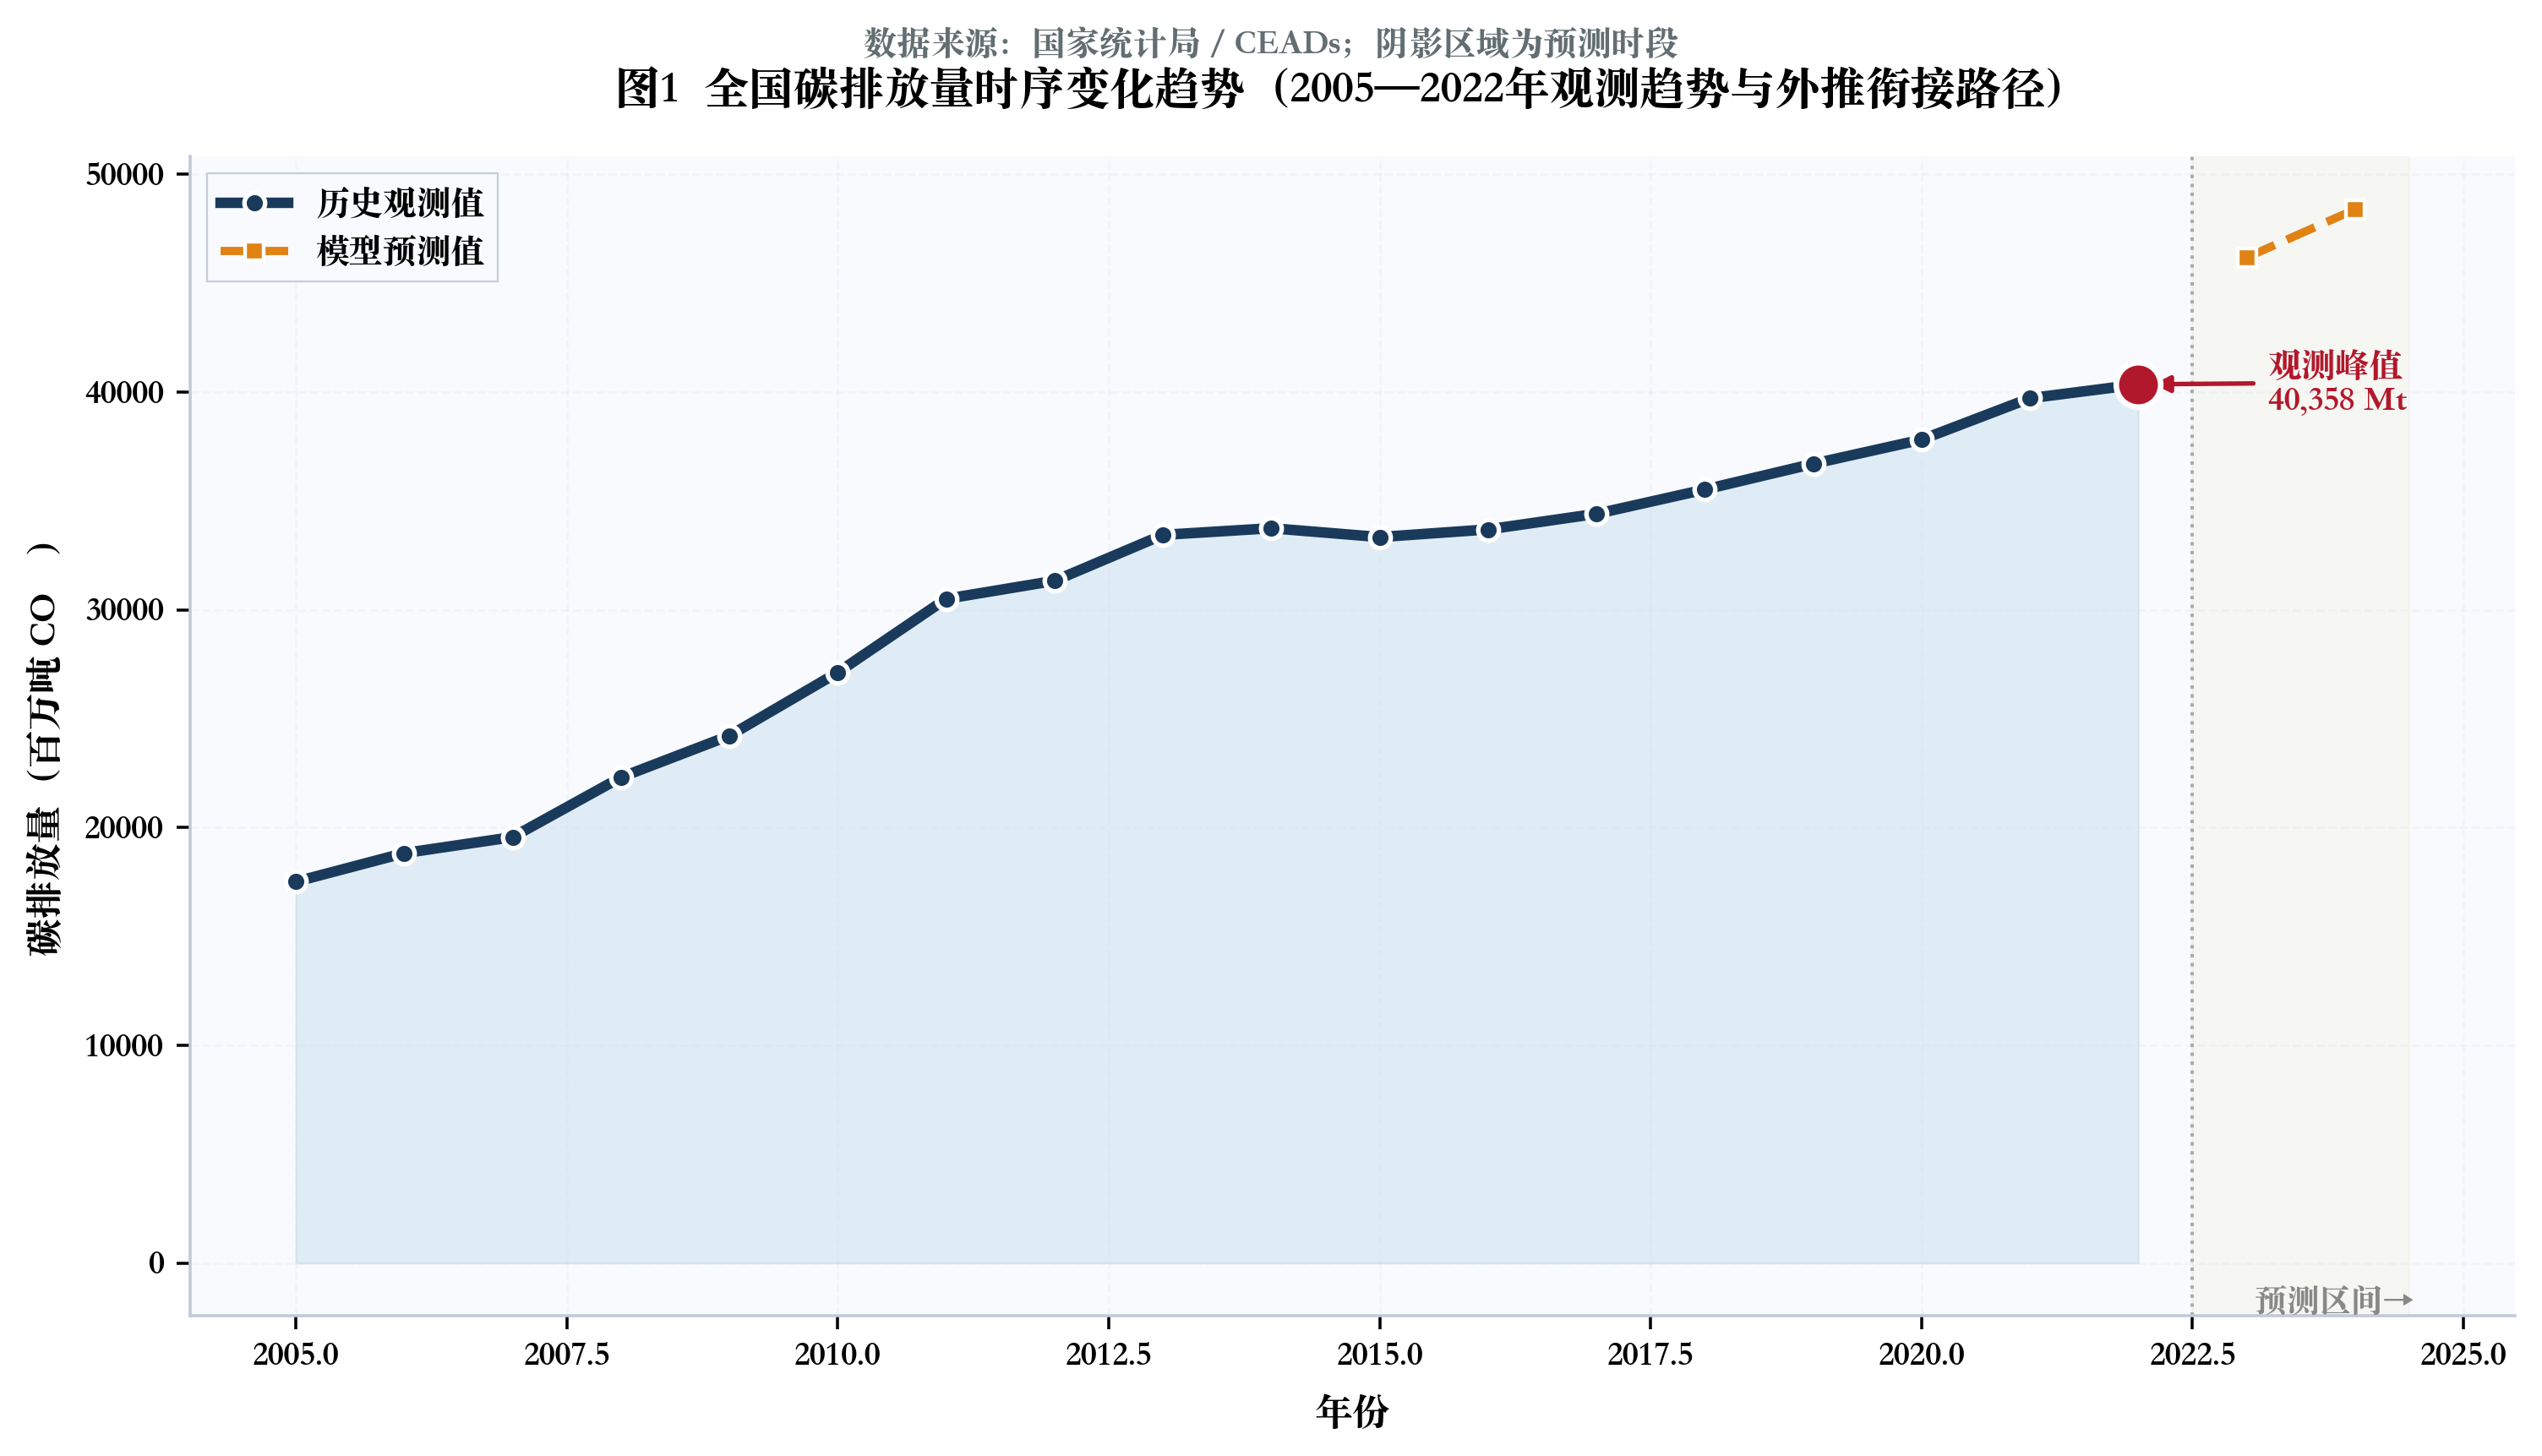
\includegraphics[width=0.82\textwidth]{../outputs/figures/Fig1_national_co2_trend.png}
    \captionof{figure}{2005—2024年中国碳排放总量变化趋势}
    \label{fig:co2_trend}
\end{center}
从图\ref{fig:co2_trend}可以看到，碳排放在样本后段仍保持上行惯性，但斜率较前期明显放缓，说明“总量扩张”与“结构调整”正在并行发生。我国排放路径已由快速爬升阶段逐步转入高位调整阶段，后续峰值形态将更受能源与产业结构变化影响。

\begin{center}
    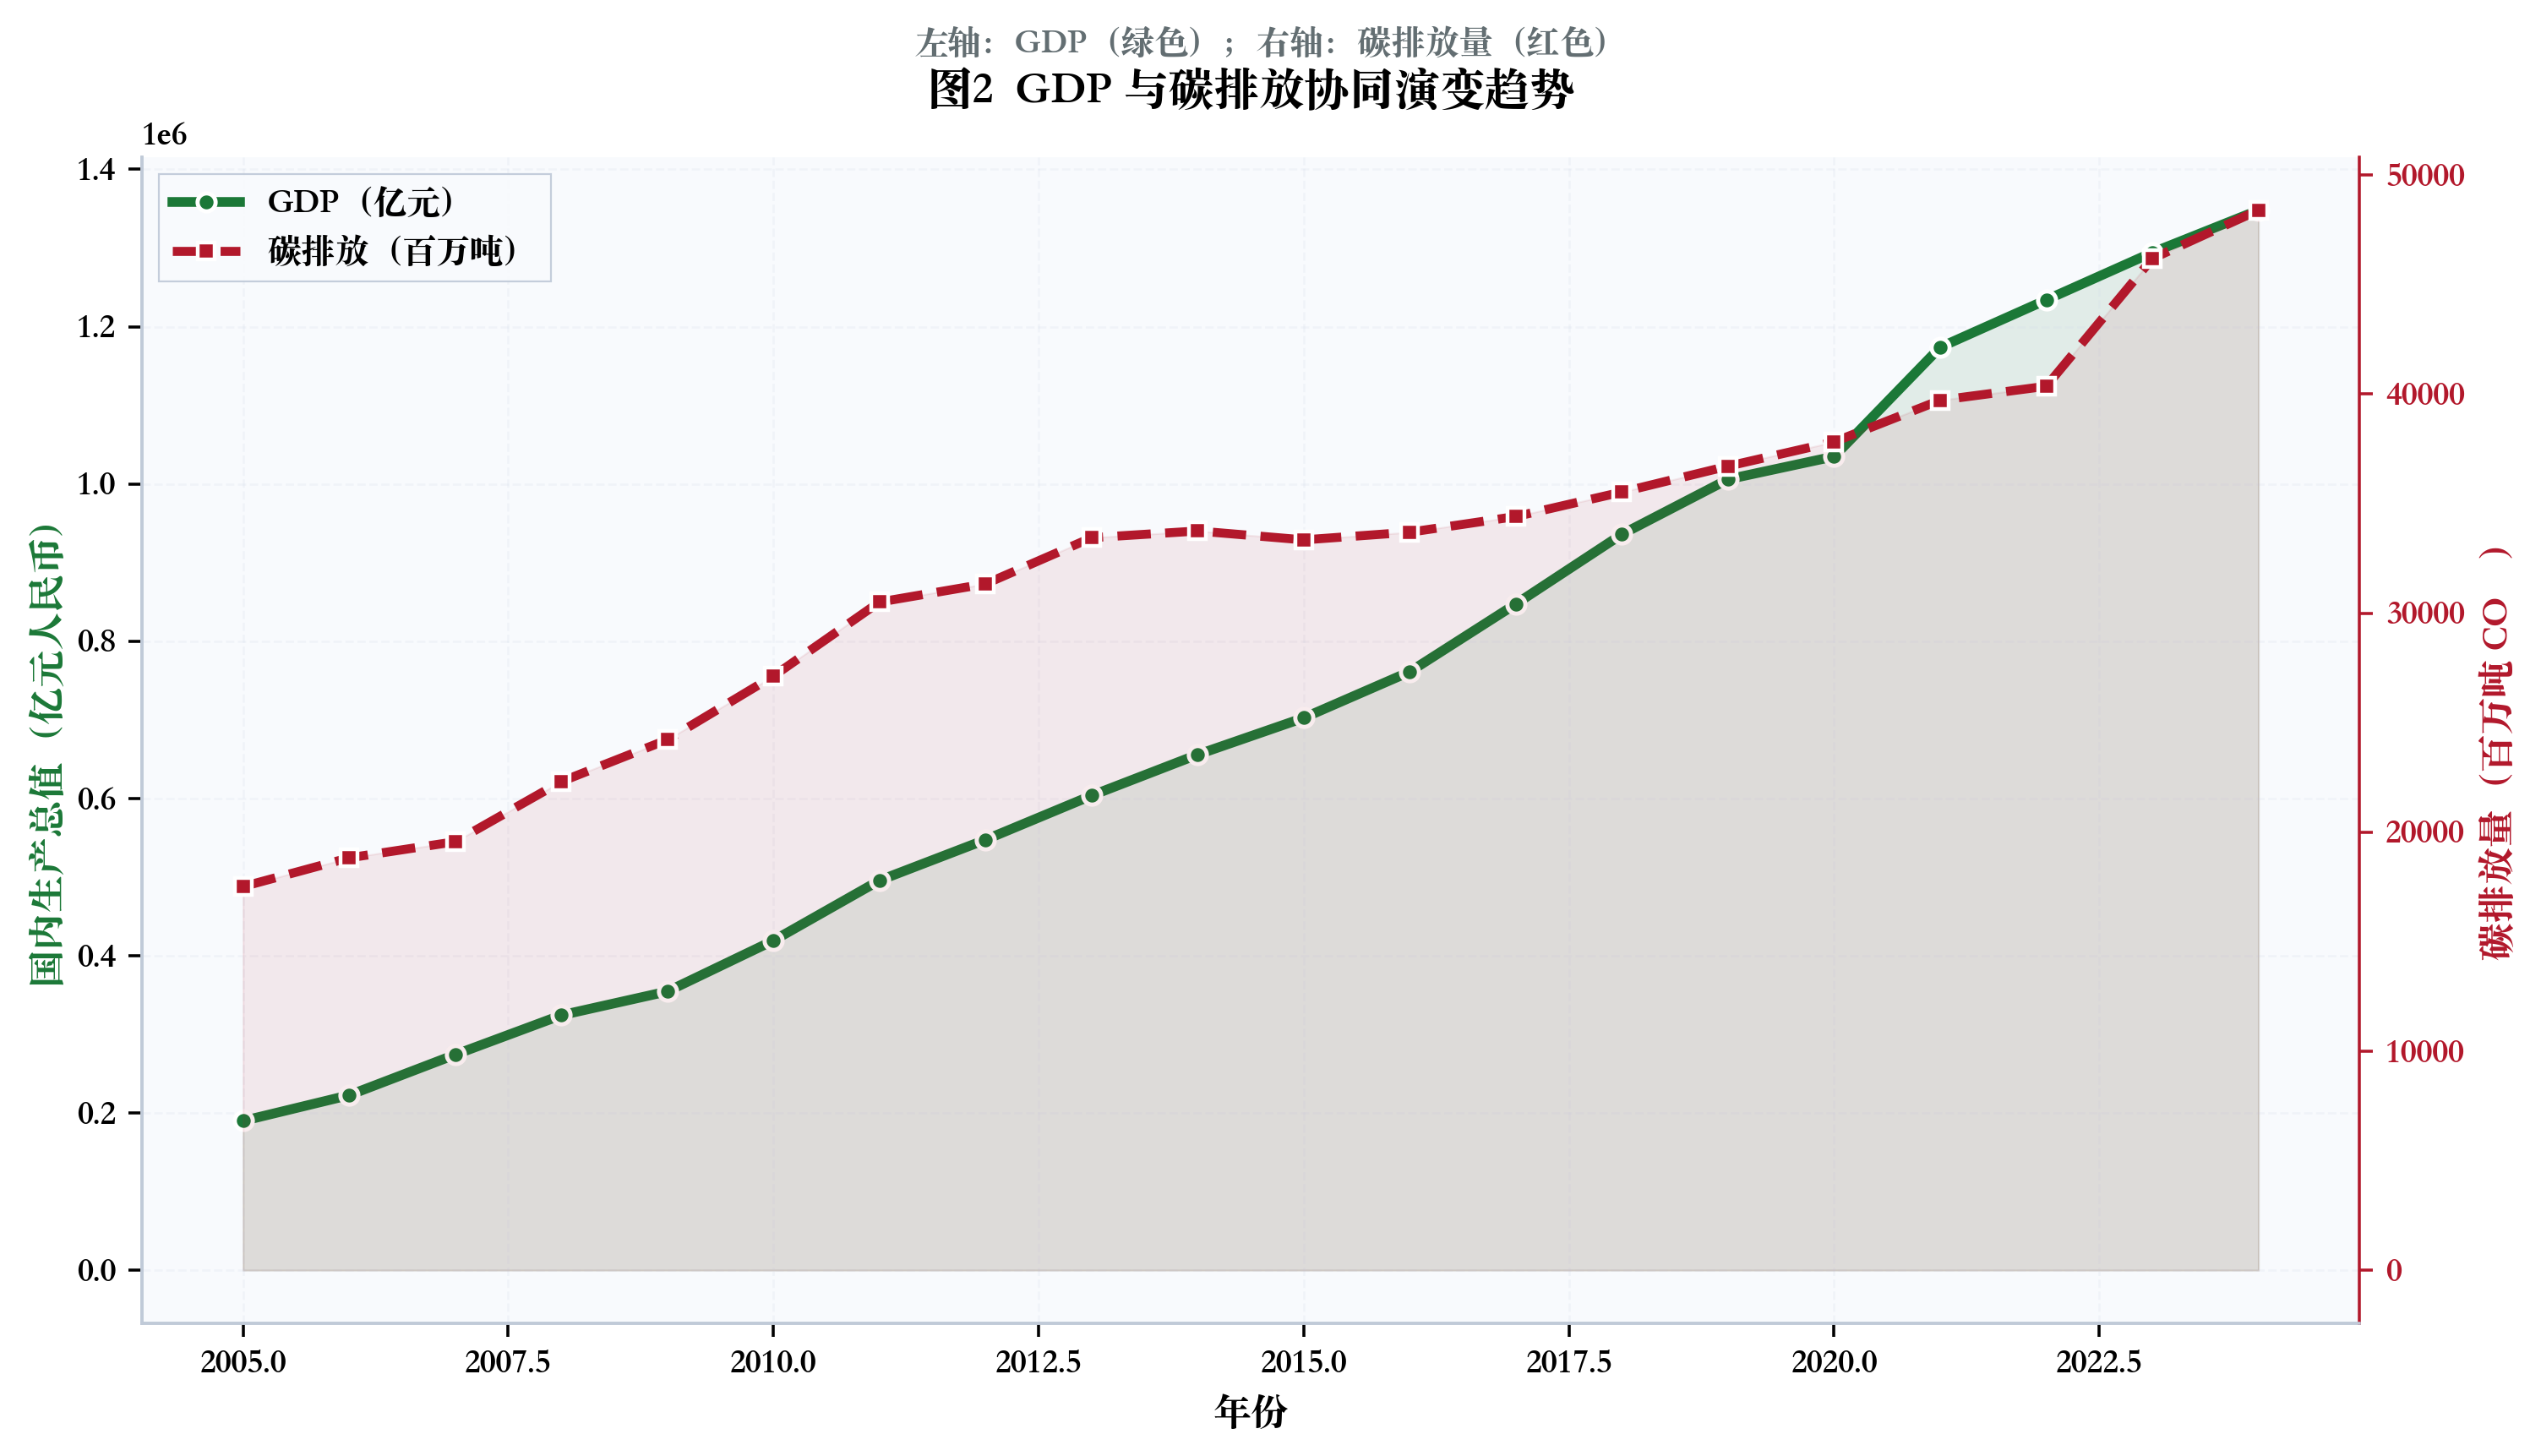
\includegraphics[width=0.86\textwidth]{../outputs/figures/Fig2_gdp_co2_dual_axis.png}
    \captionof{figure}{2005—2024年GDP与碳排放双轴对比}
    \label{fig:gdp_co2}
\end{center}
图\ref{fig:gdp_co2}表明，GDP与碳排放长期同向变化，但并非同比例同步增长。后期经济总量继续扩张而排放增速趋缓，反映增长方式正由高碳要素驱动向效率与结构驱动过渡。

\begin{center}
    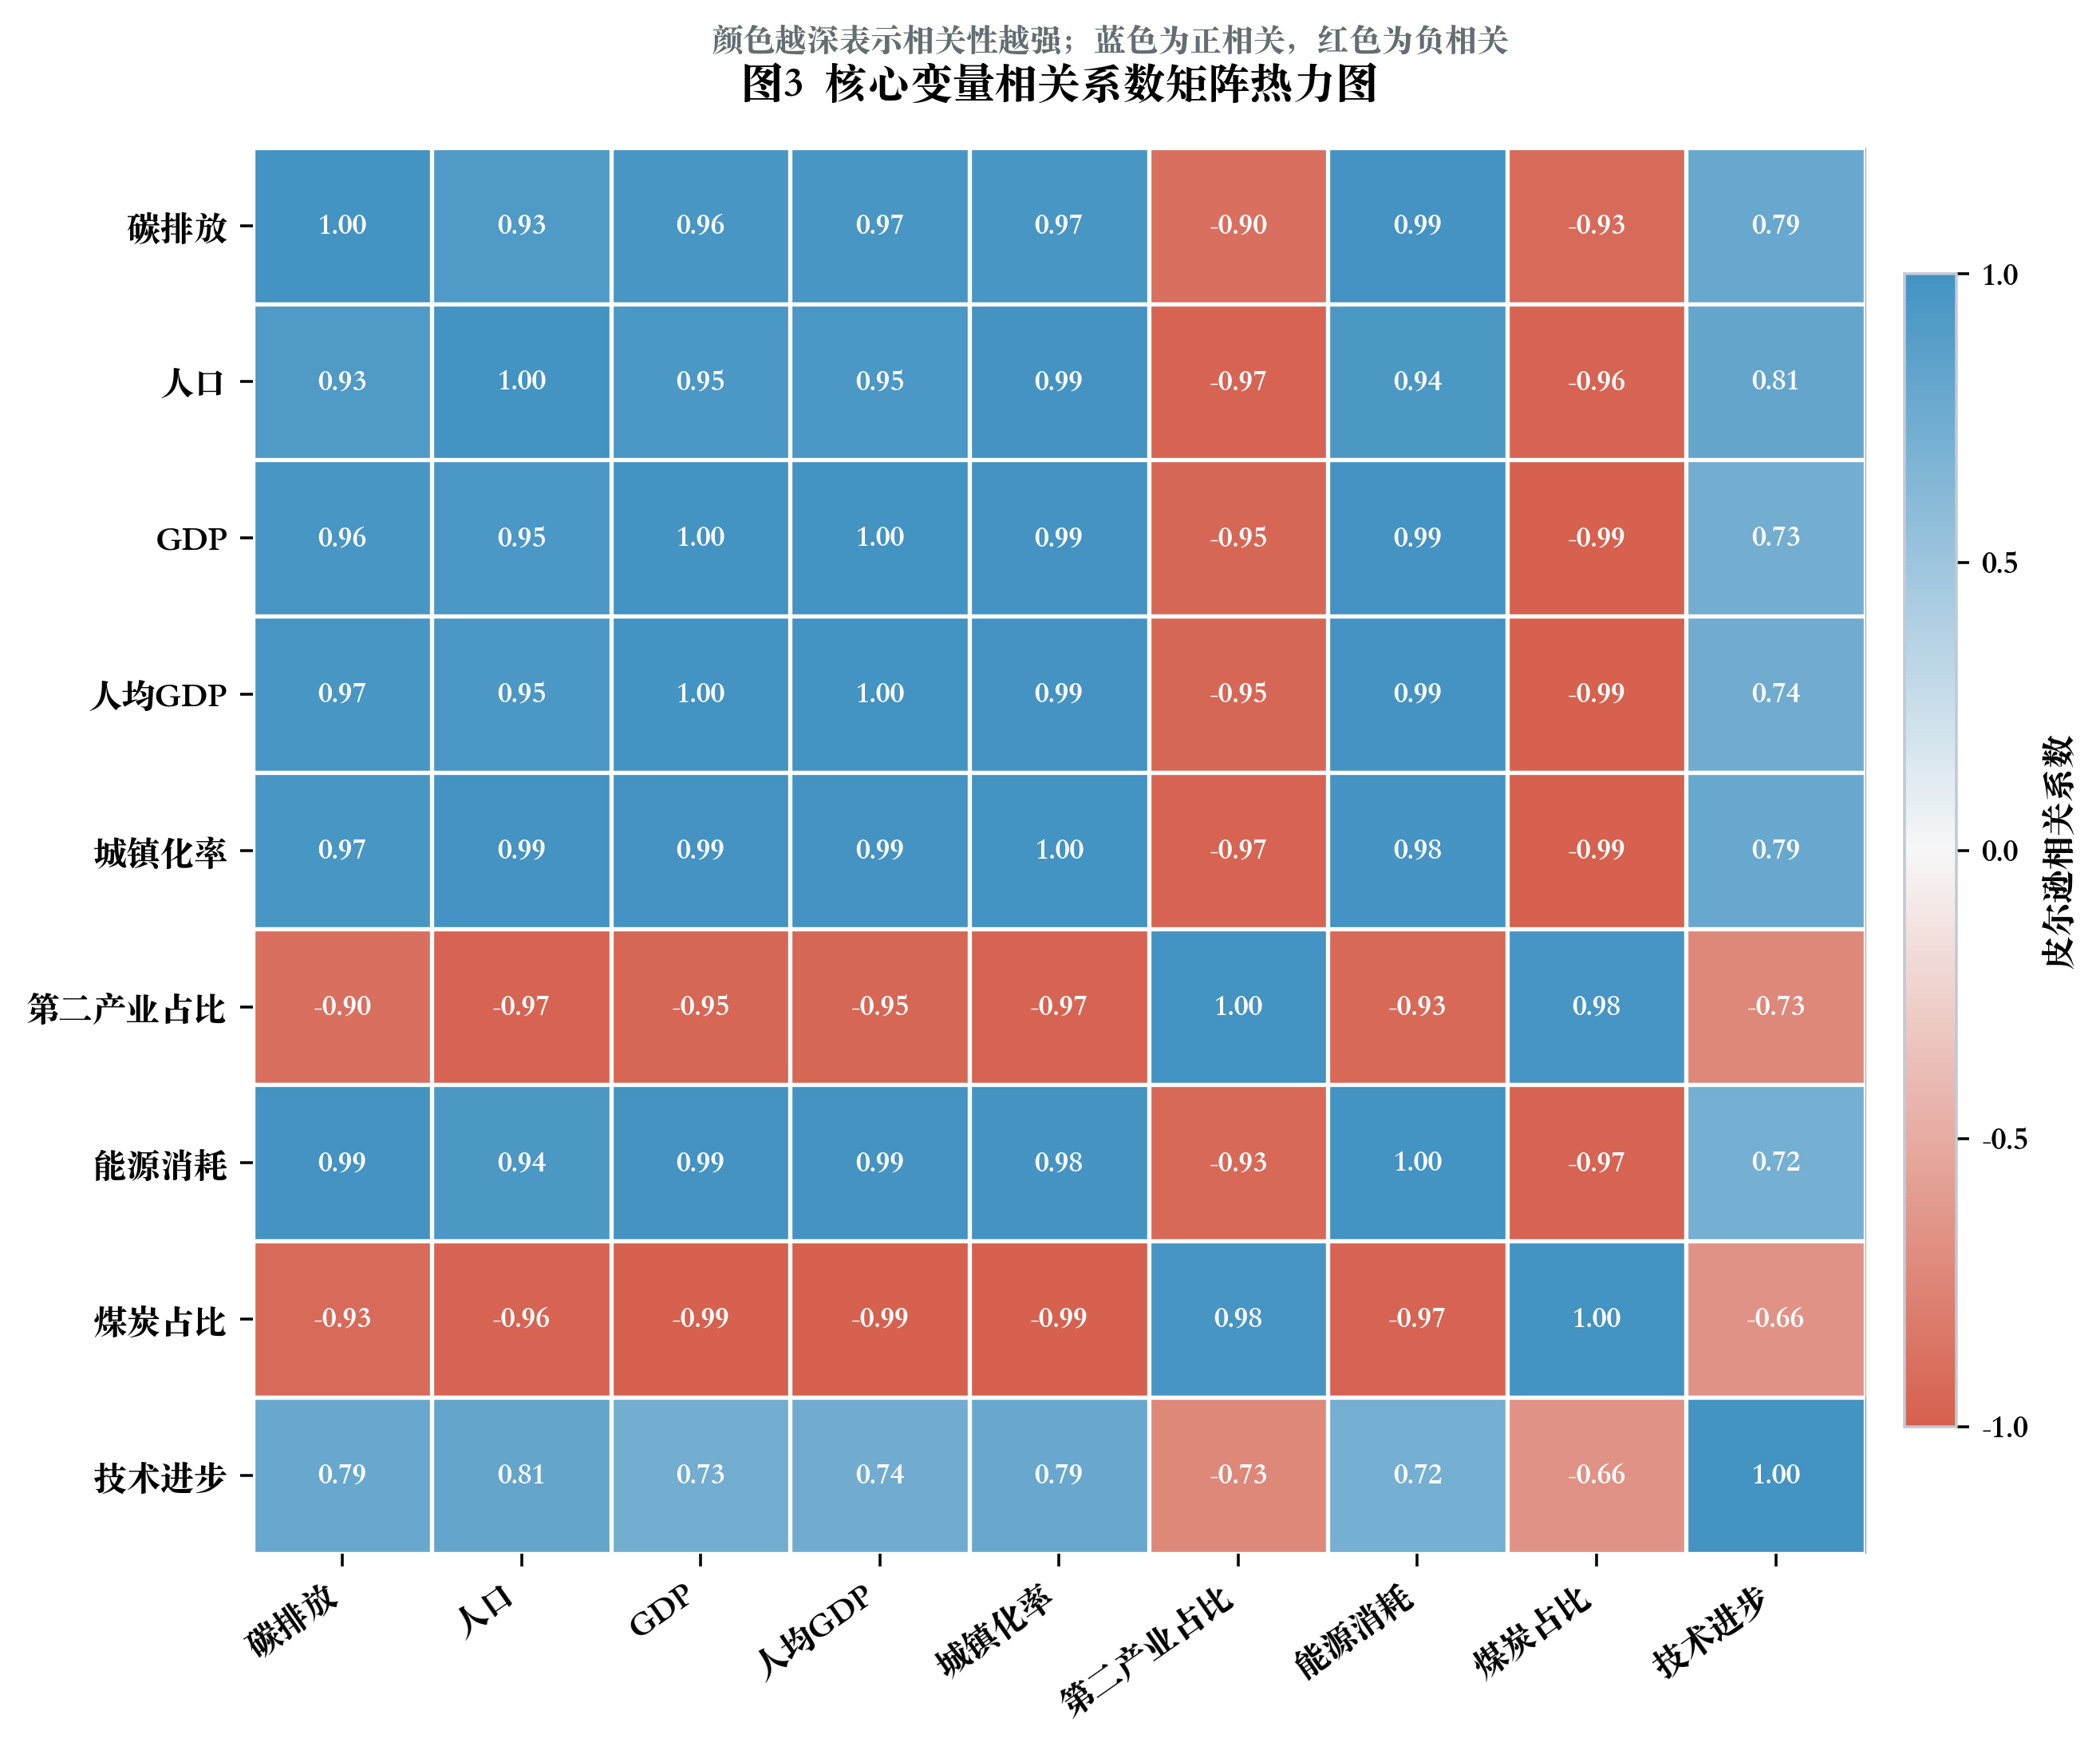
\includegraphics[width=0.78\textwidth]{../outputs/figures/Fig3_correlation_matrix.png}
    \captionof{figure}{核心变量相关性矩阵热力图}
    \label{fig:corr}
\end{center}
从图\ref{fig:corr}所示相关结构看，能源消费、GDP等规模变量与碳排放总体呈正相关；煤炭占比下降、产业升级与减排方向更一致。这一统计特征为后续参数设定提供了依据。

\begin{center}
    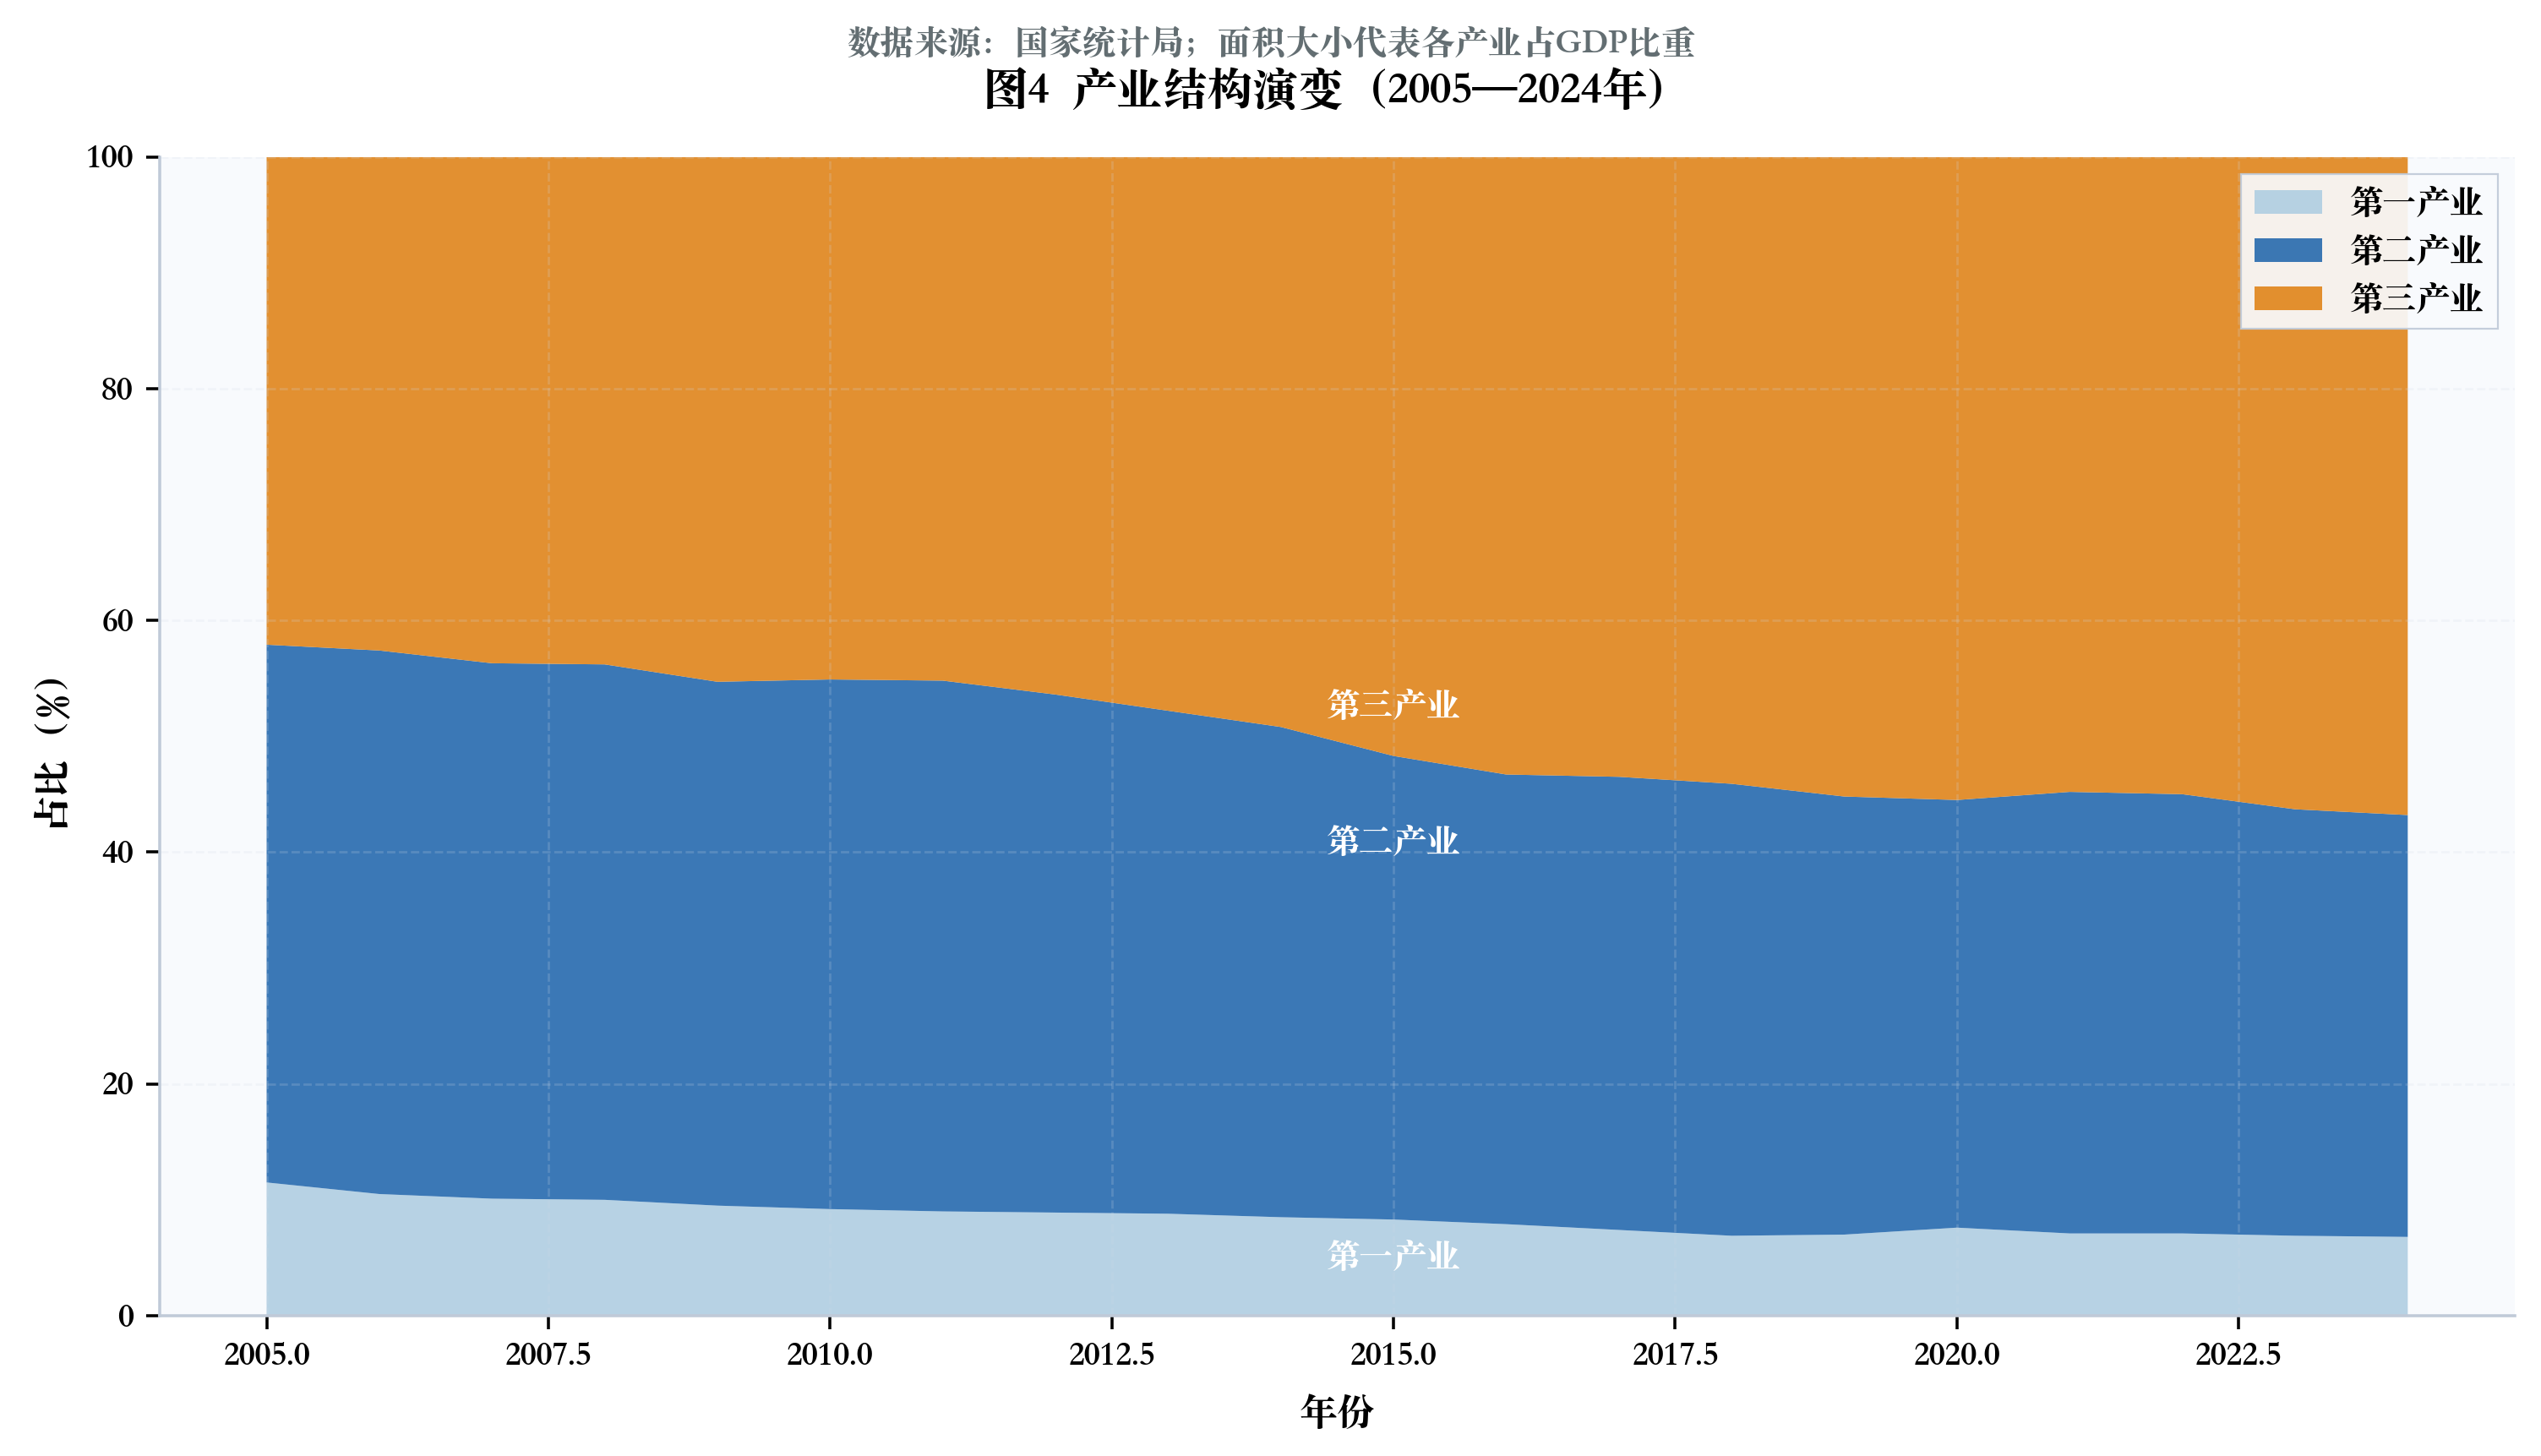
\includegraphics[width=0.84\textwidth]{../outputs/figures/Fig4_industry_structure.png}
    \captionof{figure}{产业结构演化趋势图}
    \label{fig:industry_structure}
\end{center}
结合图\ref{fig:industry_structure}可见，第二产业占比总体下降、第三产业占比上升，是样本期内排放增速放缓的重要背景。这并不意味着工业作用消失，而是说明工业内部升级与服务业扩张共同改变了单位产出对应的排放强度。

\begin{center}
    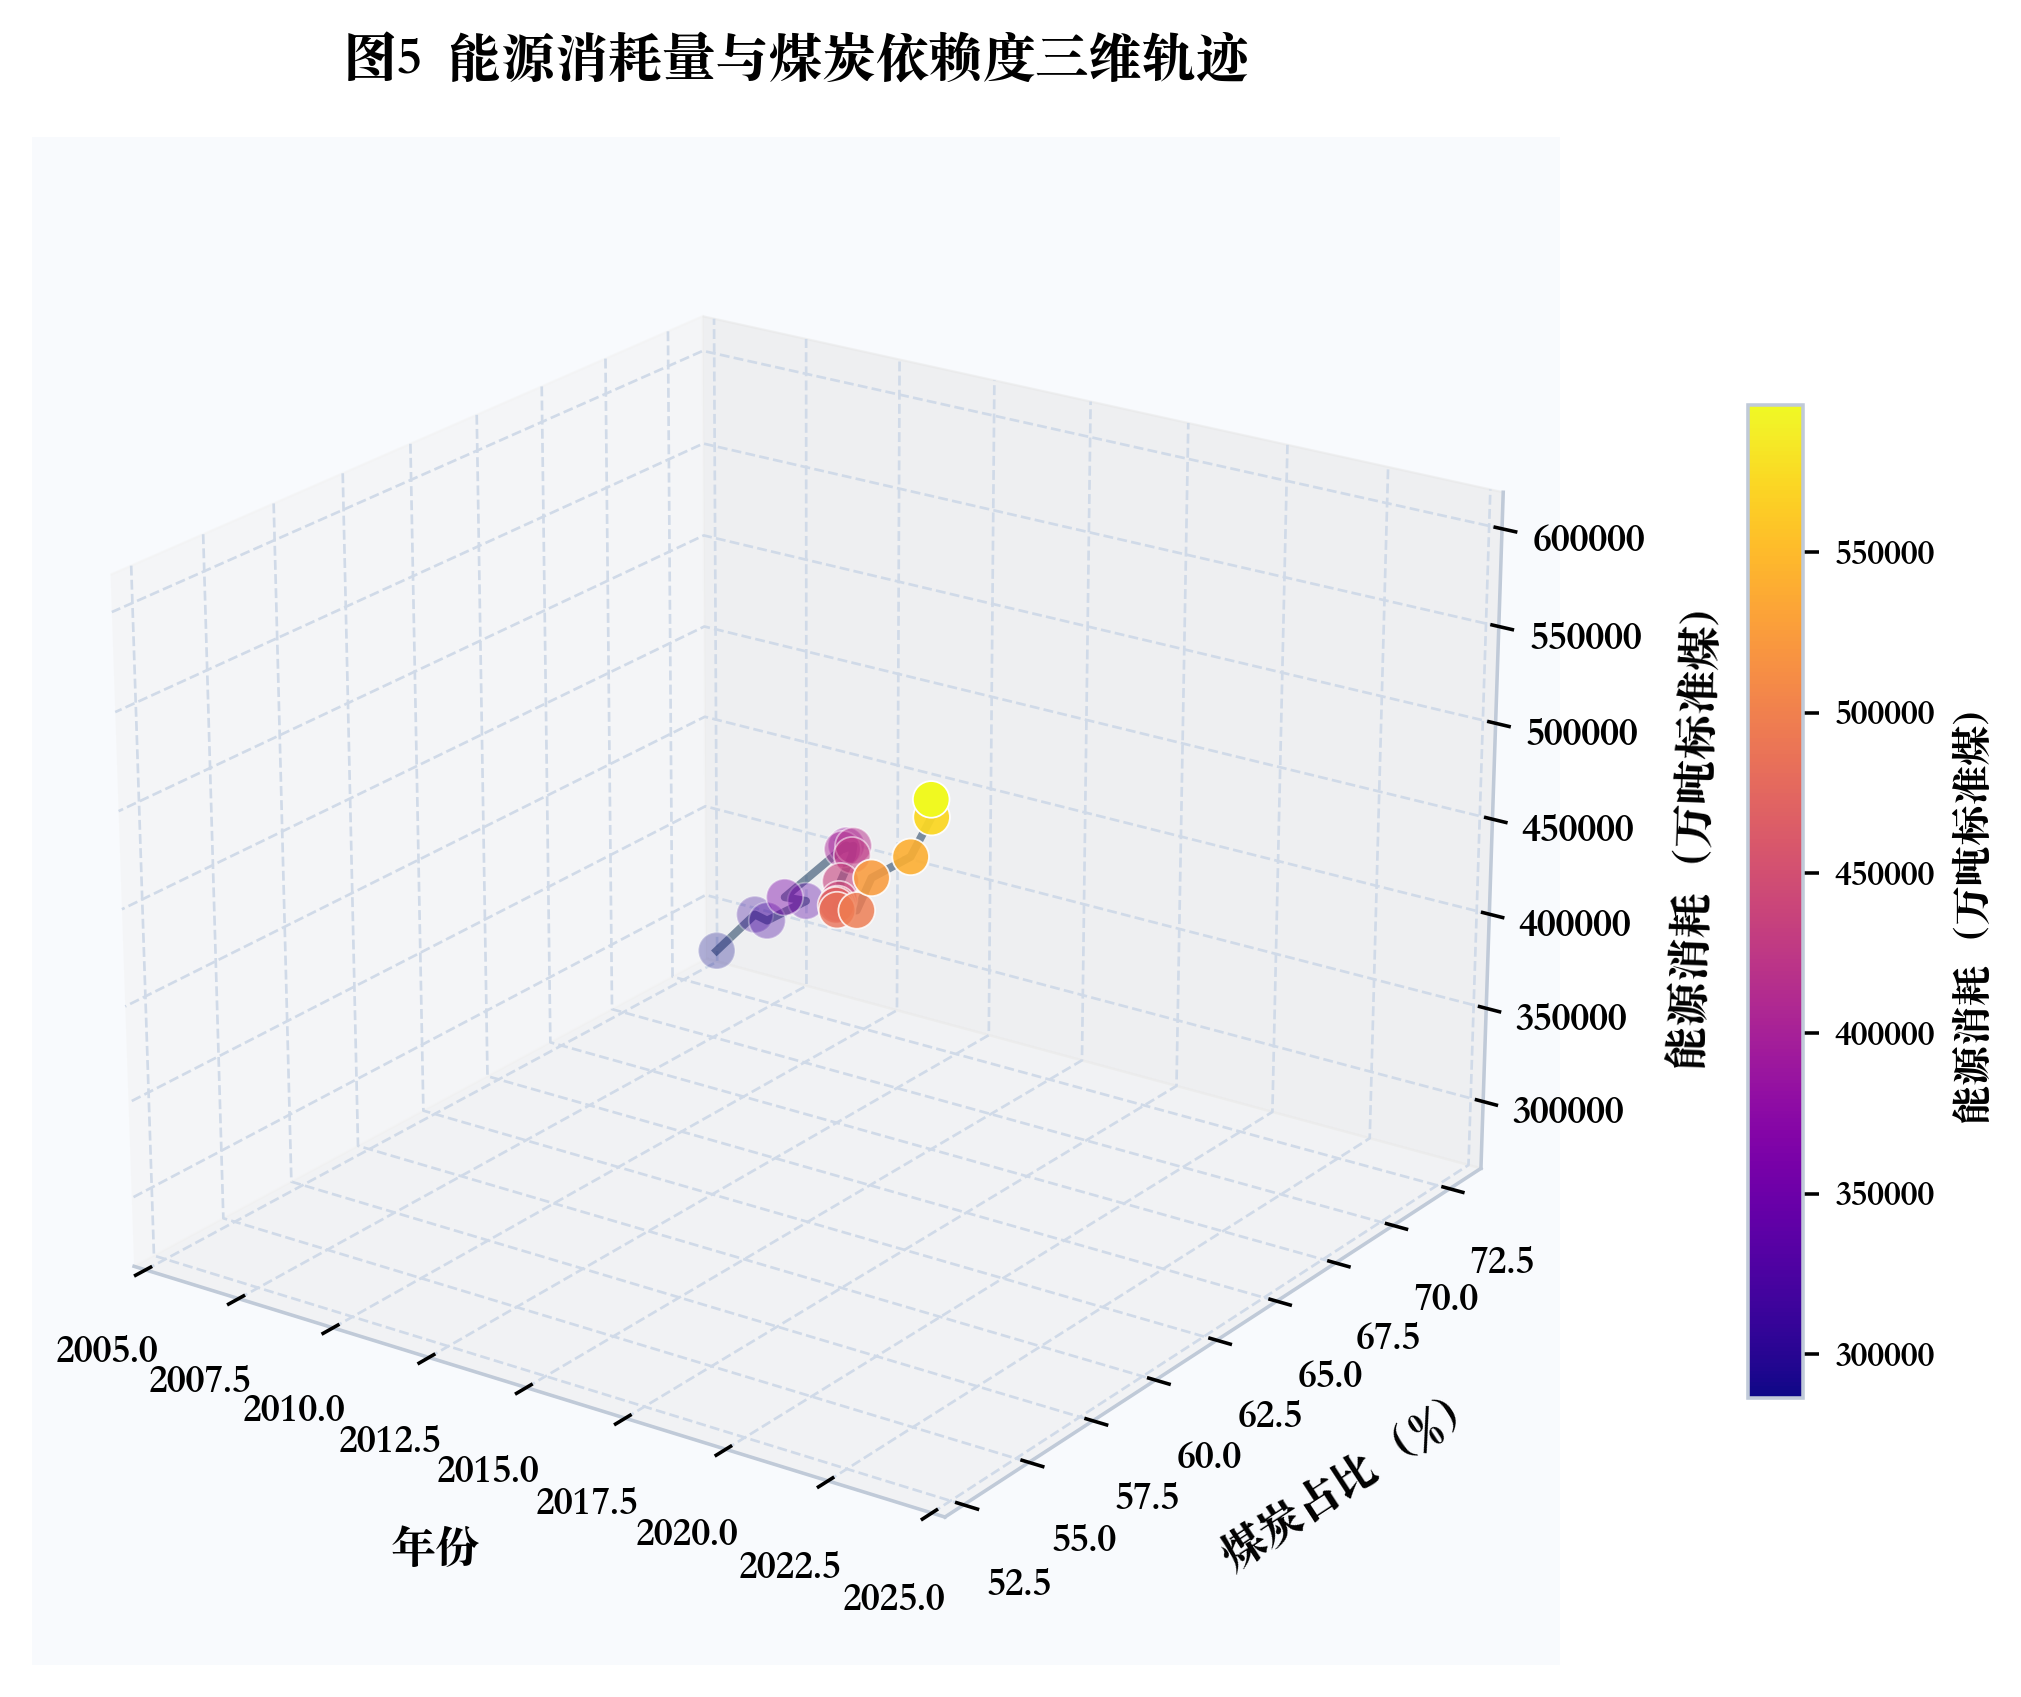
\includegraphics[width=0.82\textwidth]{../outputs/figures/Fig5_energy_structure.png}
    \captionof{figure}{能源总量与煤炭依赖三维联动图}
    \label{fig:energy_structure}
\end{center}
图\ref{fig:energy_structure}展示了“年份—煤炭依赖—能源总量”的联动关系：能源总量仍处高位，而煤炭占比持续下降。这说明我国处于“总量约束尚强、结构改善先行”的过渡阶段，也解释了为什么短期内排放难以快速下行，但中长期可通过结构优化压低峰值。

\begin{center}
    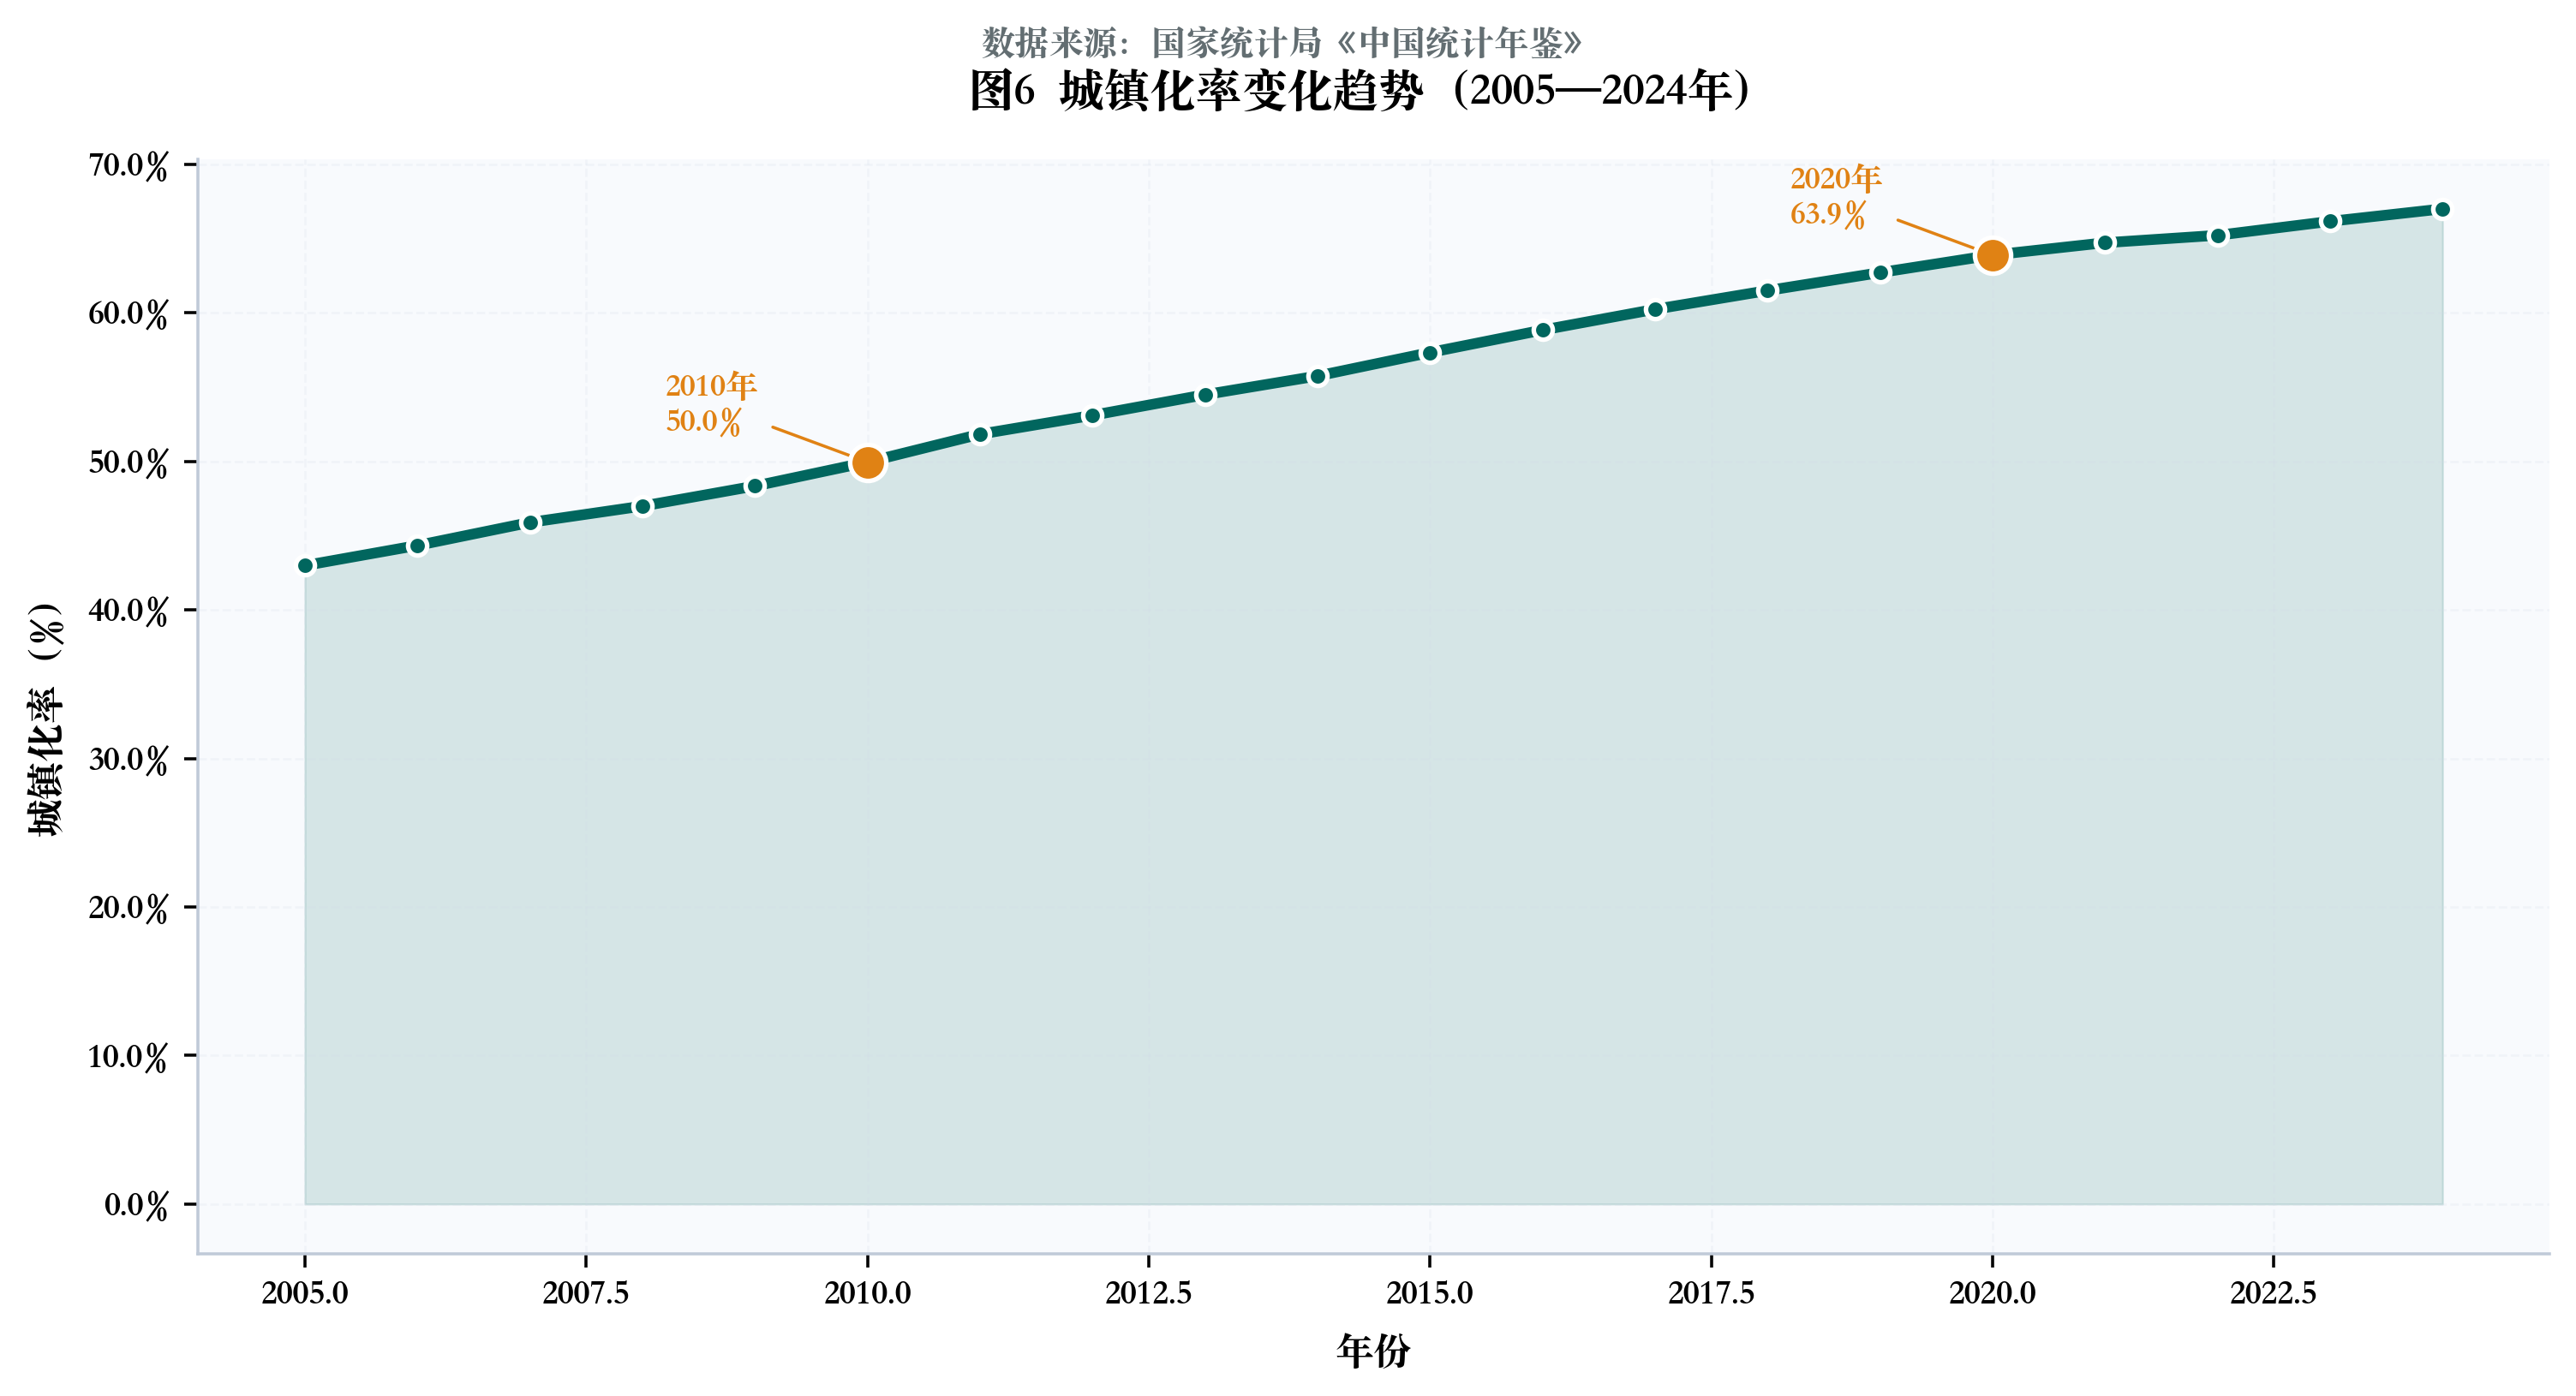
\includegraphics[width=0.82\textwidth]{../outputs/figures/Fig6_urbanization_rate.png}
    \captionof{figure}{城镇化率变化趋势}
    \label{fig:urbanization_rate}
\end{center}
由图\ref{fig:urbanization_rate}可知，城镇化率持续上升，但城镇化并不必然推高排放。若公共服务效率、基础设施集约利用和技术扩散同步提升，城镇化可能转化为减排效率提升通道。

\subsection{驱动机制识别}
在总体趋势基础上，本节通过EKC检验、扩展STIRPAT估计和中介分析识别“经济—能源—结构—技术”的作用链。

\begin{center}
    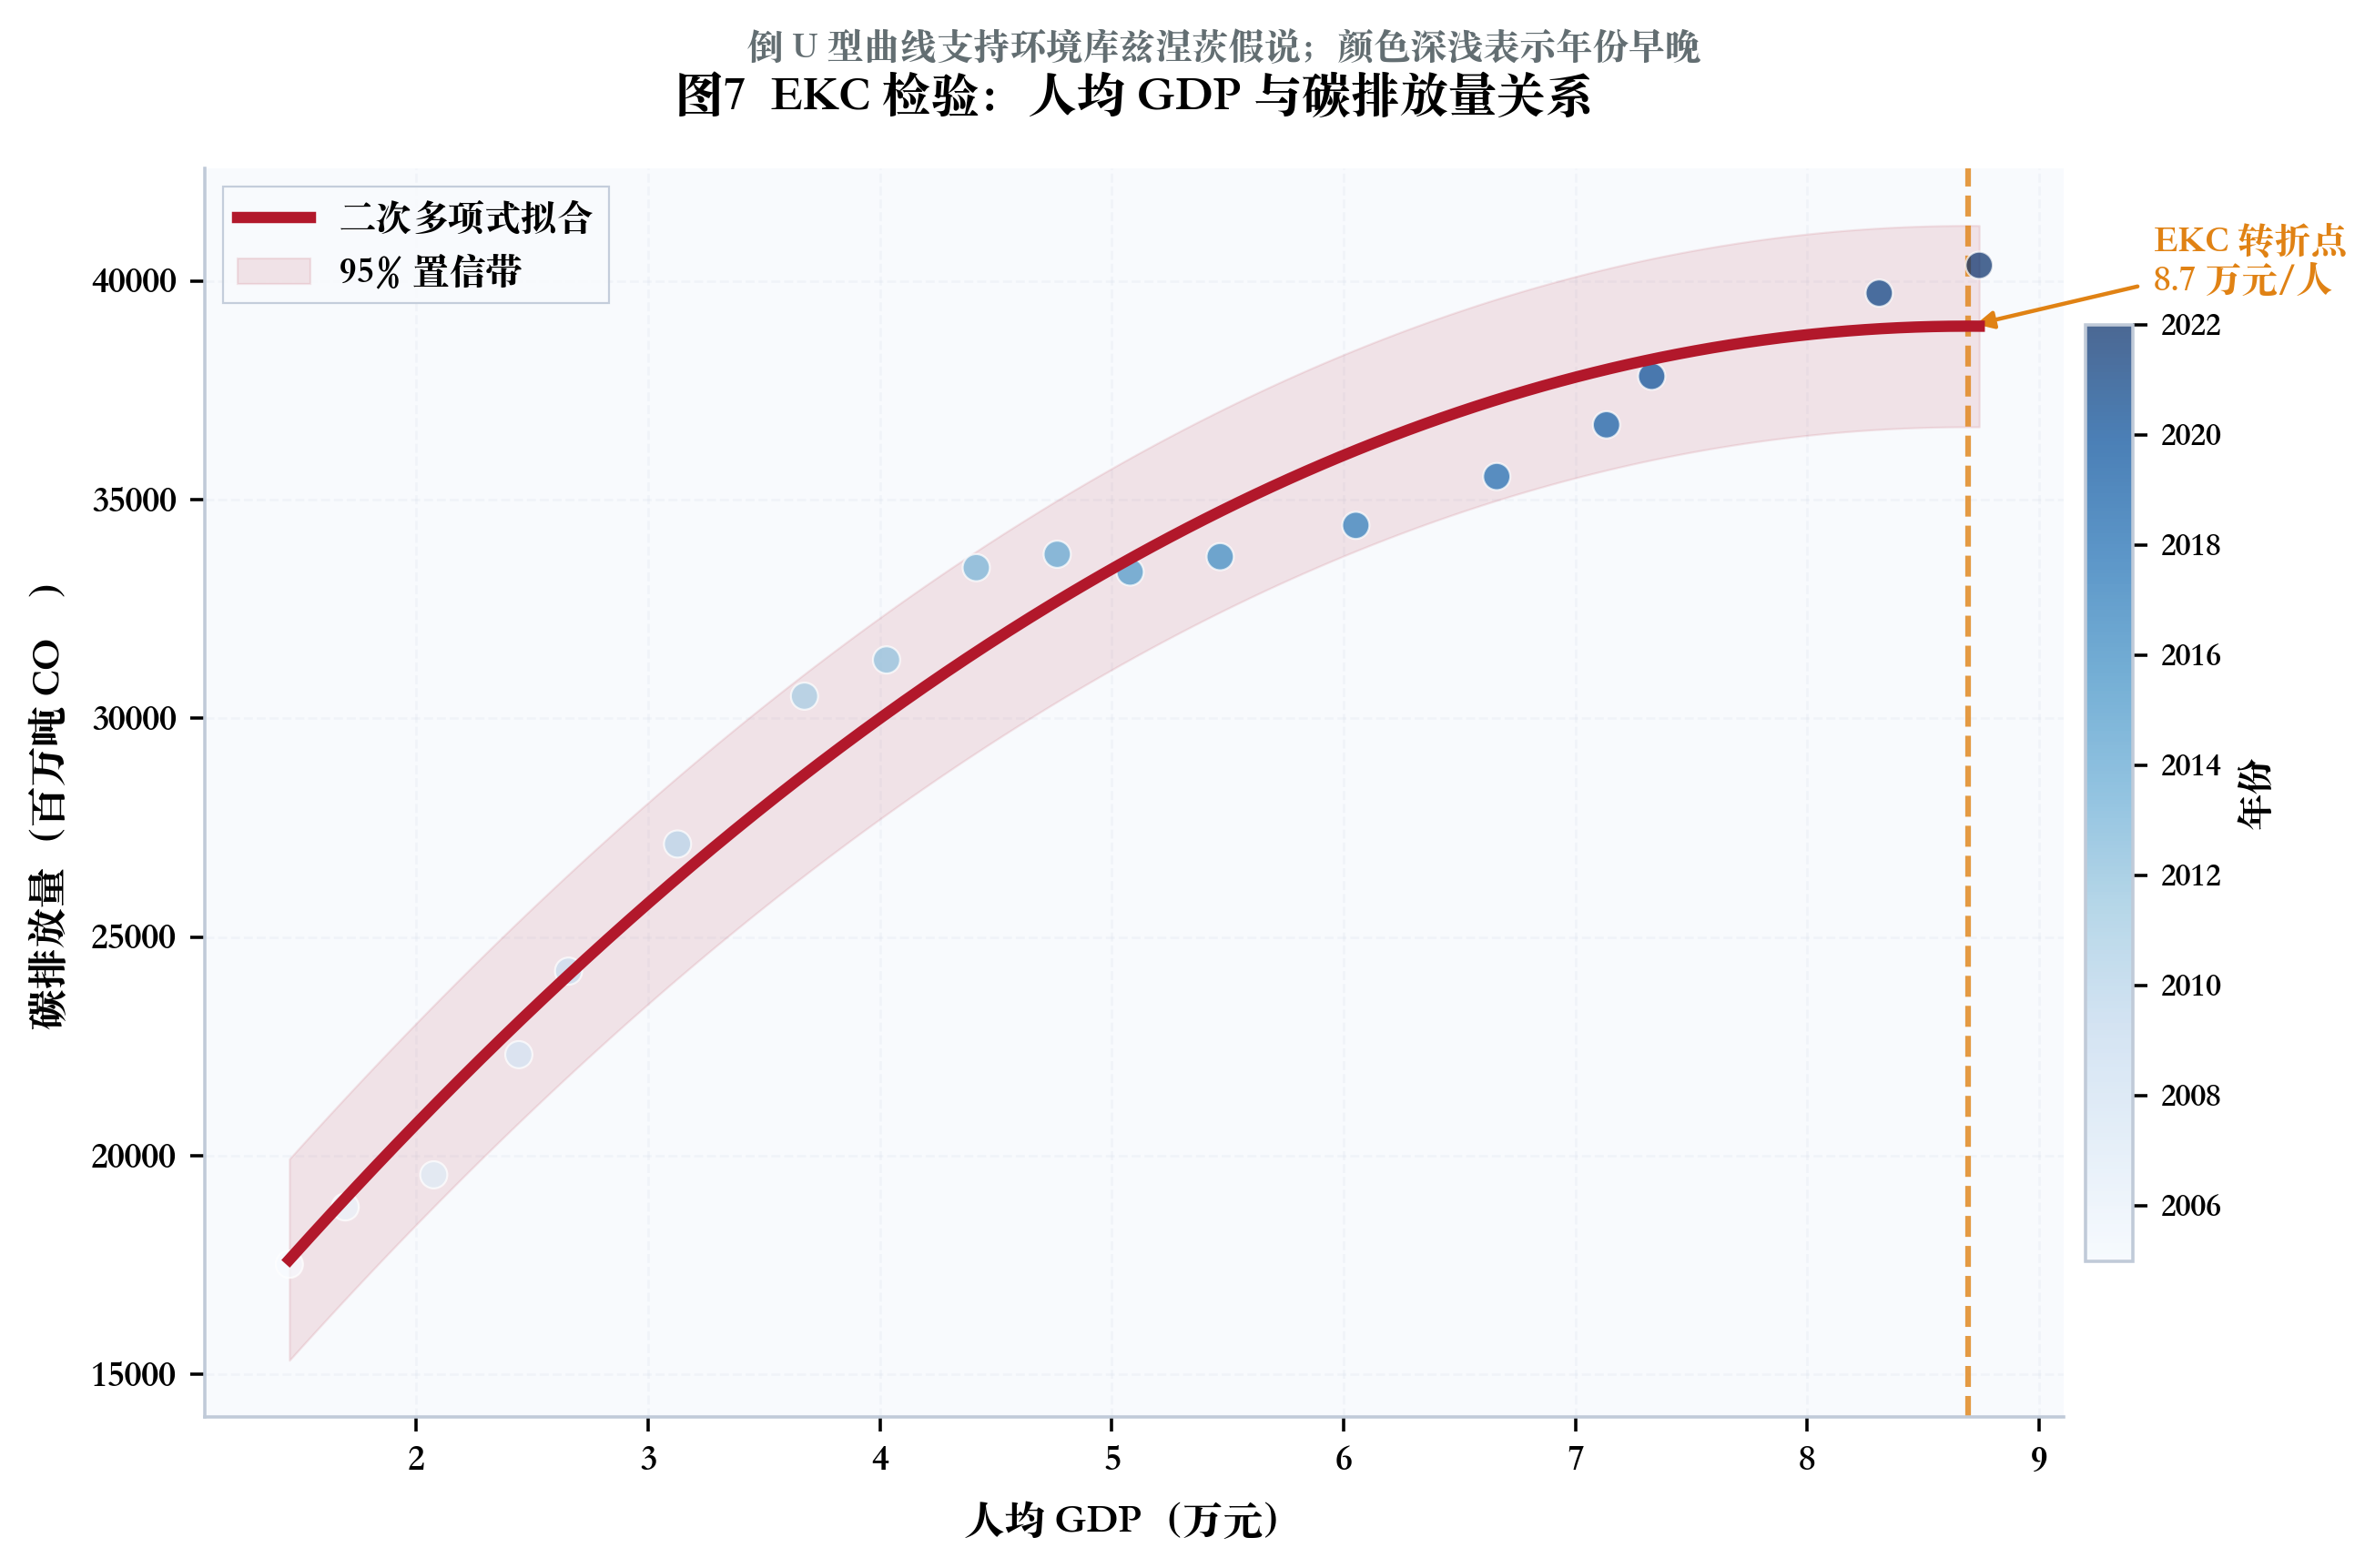
\includegraphics[width=0.72\textwidth]{../outputs/figures/Fig7_ekc_scatter_fit.png}
    \captionof{figure}{EKC检验：人均GDP与碳排放关系}
    \label{fig:ekc}
\end{center}
从图\ref{fig:ekc}可以看出，人均GDP与碳排放之间存在显著非线性关系，说明排放演化并非简单线性过程，而是进入受产业升级与能源替代共同影响的阶段性转型区间。


\begin{center}
    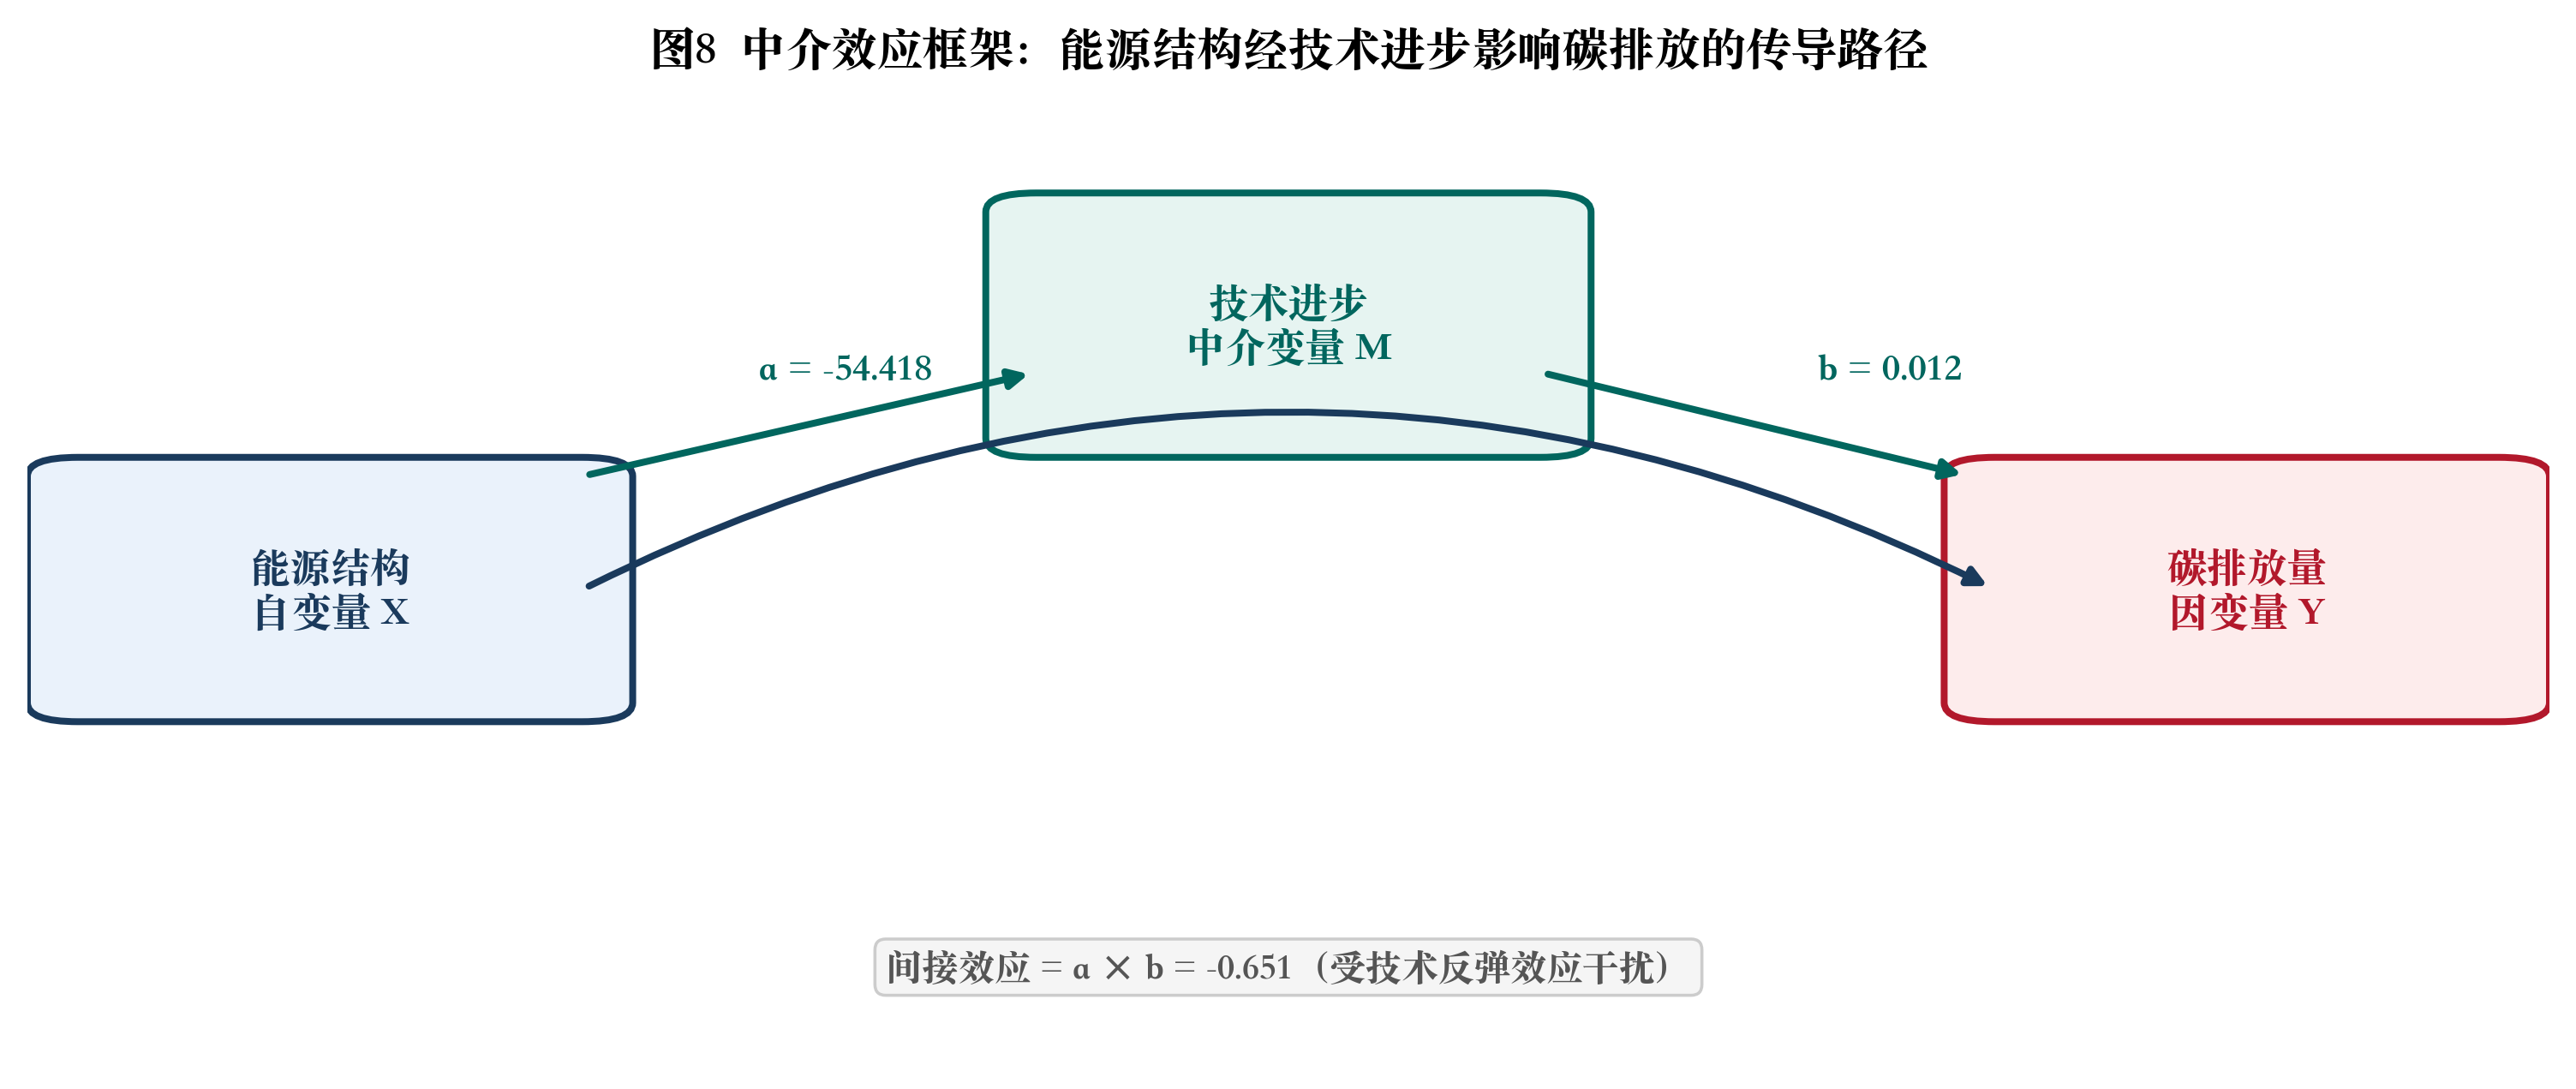
\includegraphics[width=0.84\textwidth]{../outputs/figures/Fig8_mediation_framework.png}
    \captionof{figure}{中介效应路径示意图}
    \label{fig:mediation}
\end{center}
图\ref{fig:mediation}揭示了能源结构对碳排放的复杂传导路径。值得注意的是，在未控制经济规模的单方程回归中，煤炭占比的总效应系数呈负向。这主要是受样本期内GDP与煤炭占比反向变动趋势的干扰。在剥离规模效应后，其直接效应转为显著正向，这进一步说明了前文扩展 STIRPAT 模型中多变量联合控制的必要性。

从中介链条来看，煤炭占比对技术进步（a 路径）具有显著的负向压制（$a = -54.42$），说明高煤耗路径在一定程度上挤出了创新要素积累；而技术进步对排放的影响（b 路径）在控制 GDP 后表现为极微弱的正向（$b = 0.012$），间接效应（$a \times b = -0.65$）虽为负，但绝对量远小于直接效应。这表明，能源替代的核心减排逻辑在于直接压降高碳底座（$c'$ 路径），而非依赖间接的技术创新传导，该结果为``以能源结构调整为绝对主抓手''的政策导向提供了严谨的计量证据。

\begin{center}
    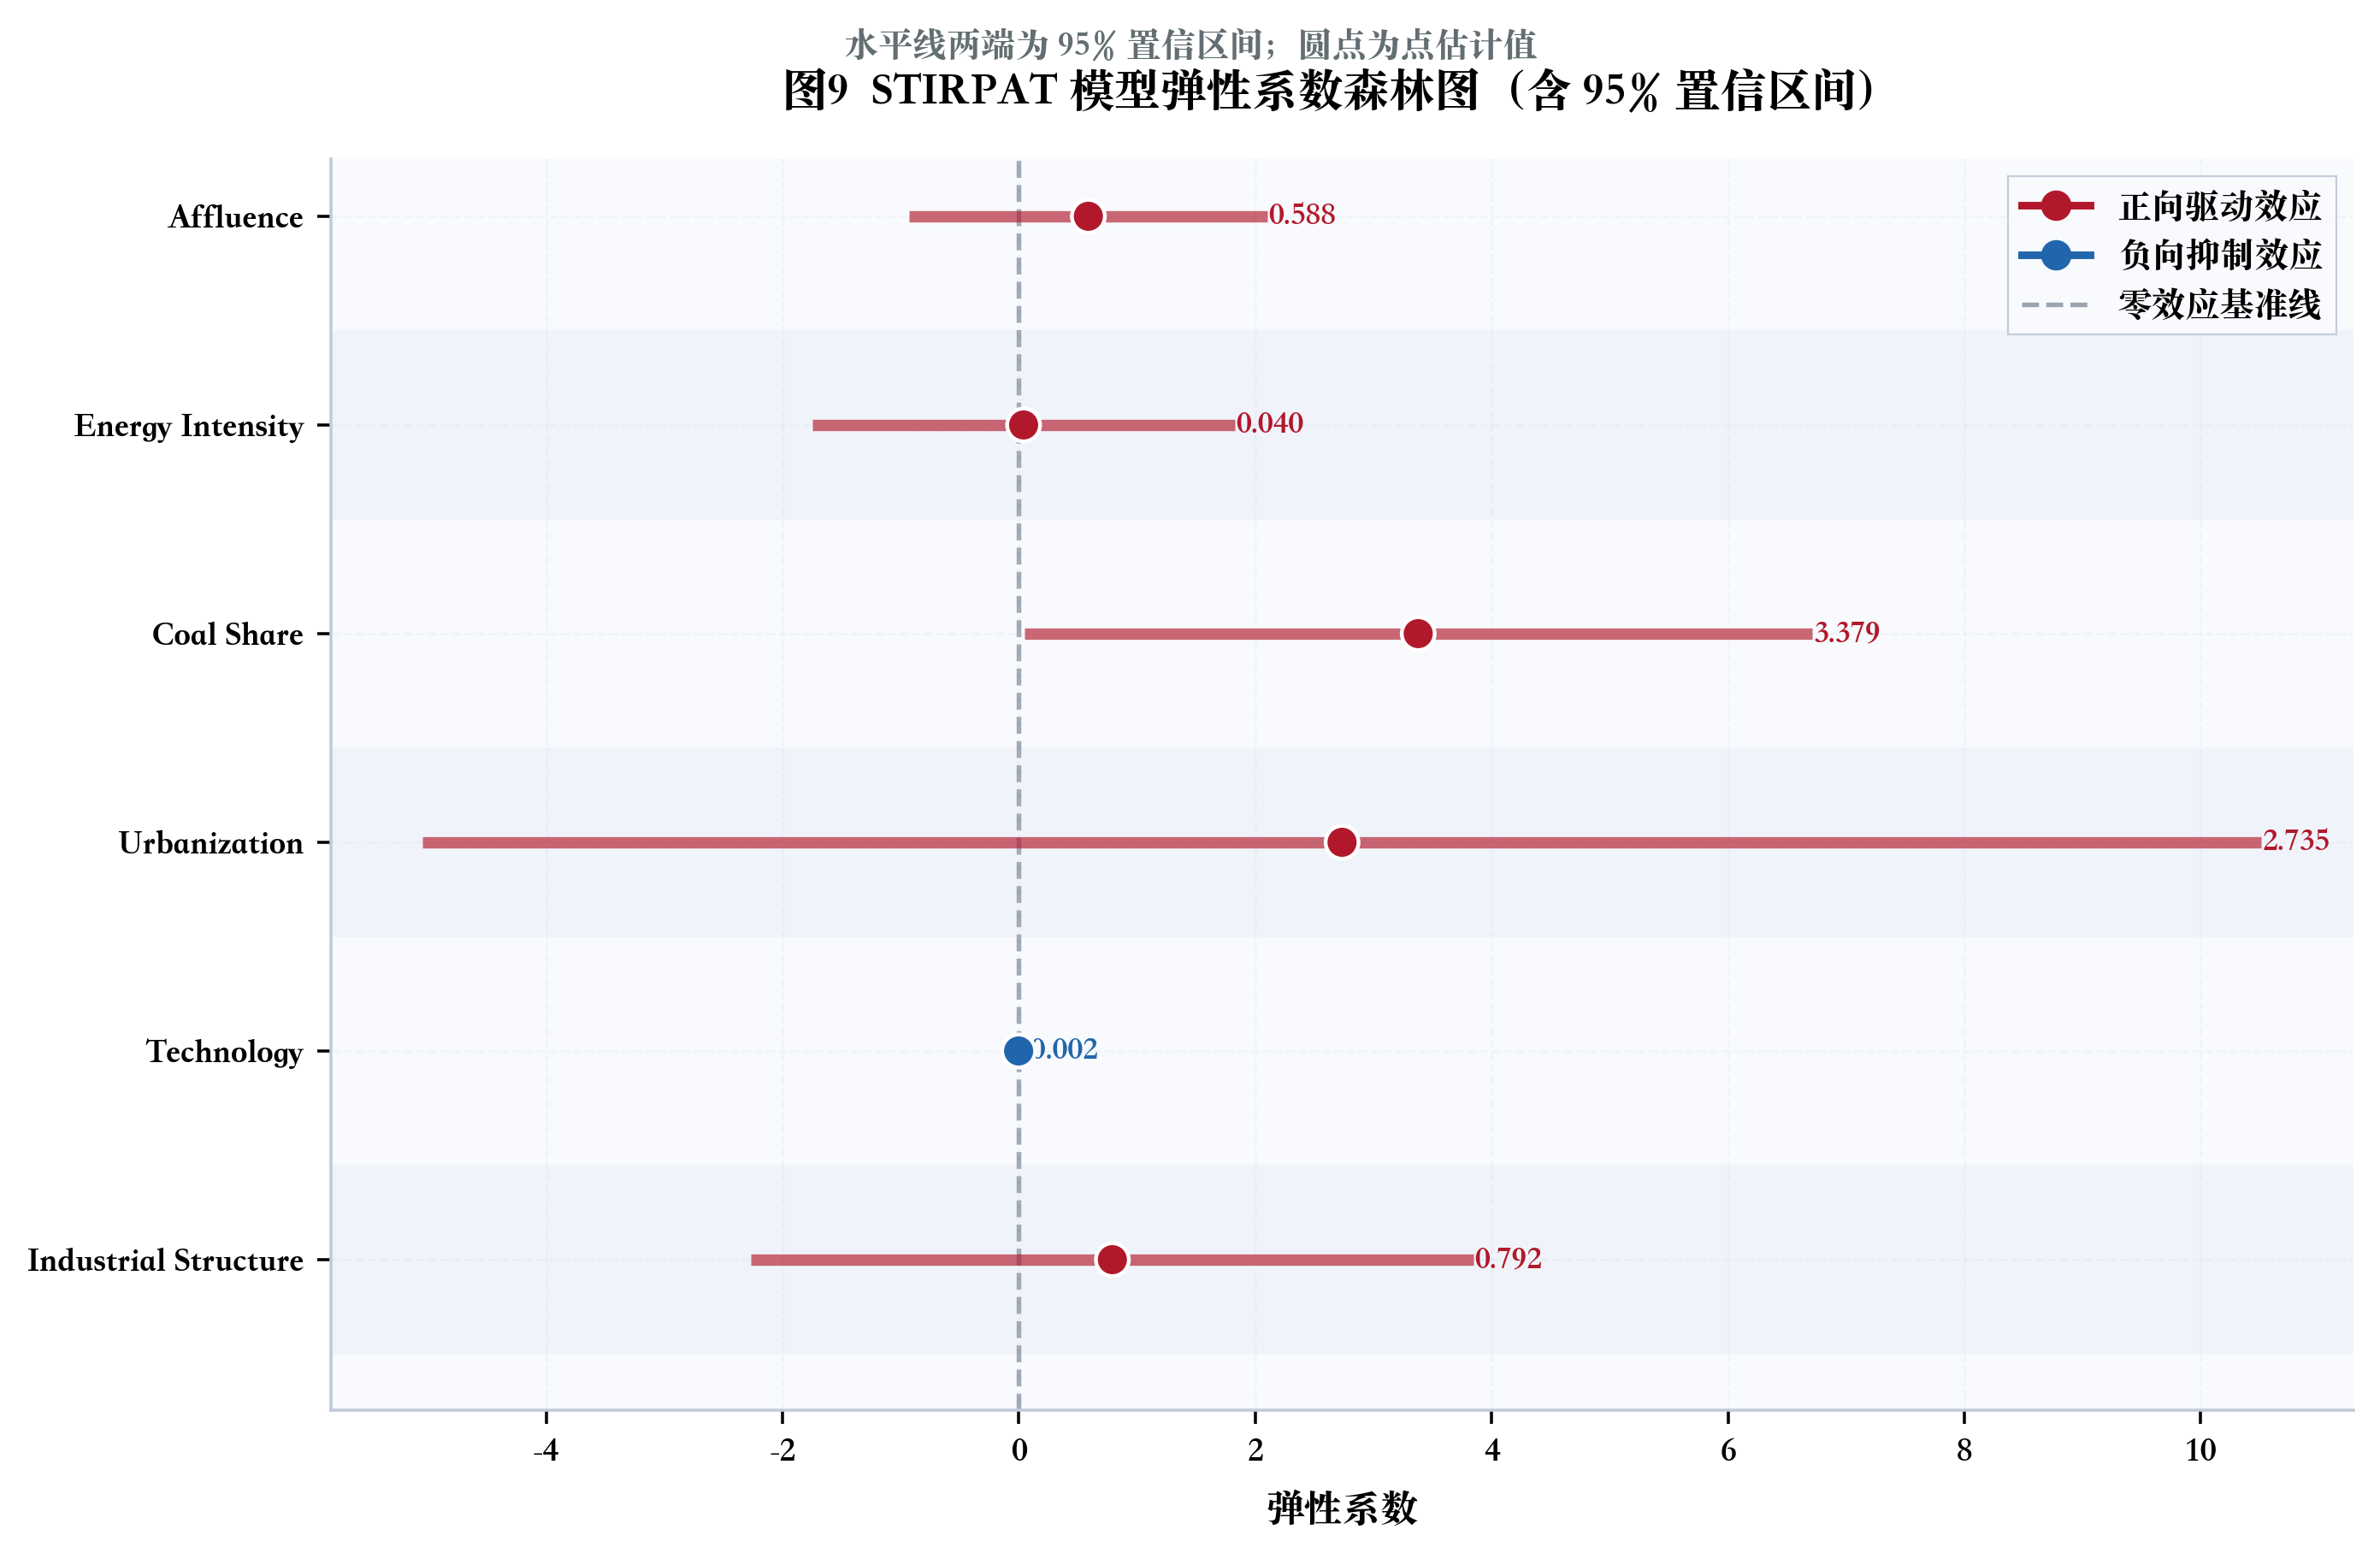
\includegraphics[width=0.78\textwidth]{../outputs/figures/Fig9_stirpat_coefficients.png}
    \captionof{figure}{扩展STIRPAT关键弹性系数图}
    \label{fig:stirpat}
\end{center}
图\ref{fig:stirpat}对应结果显示，在2005—2022年观测样本（18期）下，扩展STIRPAT回归需估计6个解释变量和截距项，共7个参数，自由度仅约11。受限于样本长度与小样本估计不确定性，系数区间普遍较宽。结果表明，仅煤炭占比在95\%置信水平下保持显著正向影响（弹性约3.3791，95\%置信区间[0.0469,\,6.7112]），是统计上最稳健的驱动因子；人均GDP、能源强度、城镇化和产业结构等变量虽点估计多为正，但置信区间包含零，未达到统计显著。这说明小样本条件下难以稳定识别其边际效应强度，但并不否定其经济机制上的现实作用，后续需通过延长样本期或进一步精简变量提高识别精度。

\begin{center}
    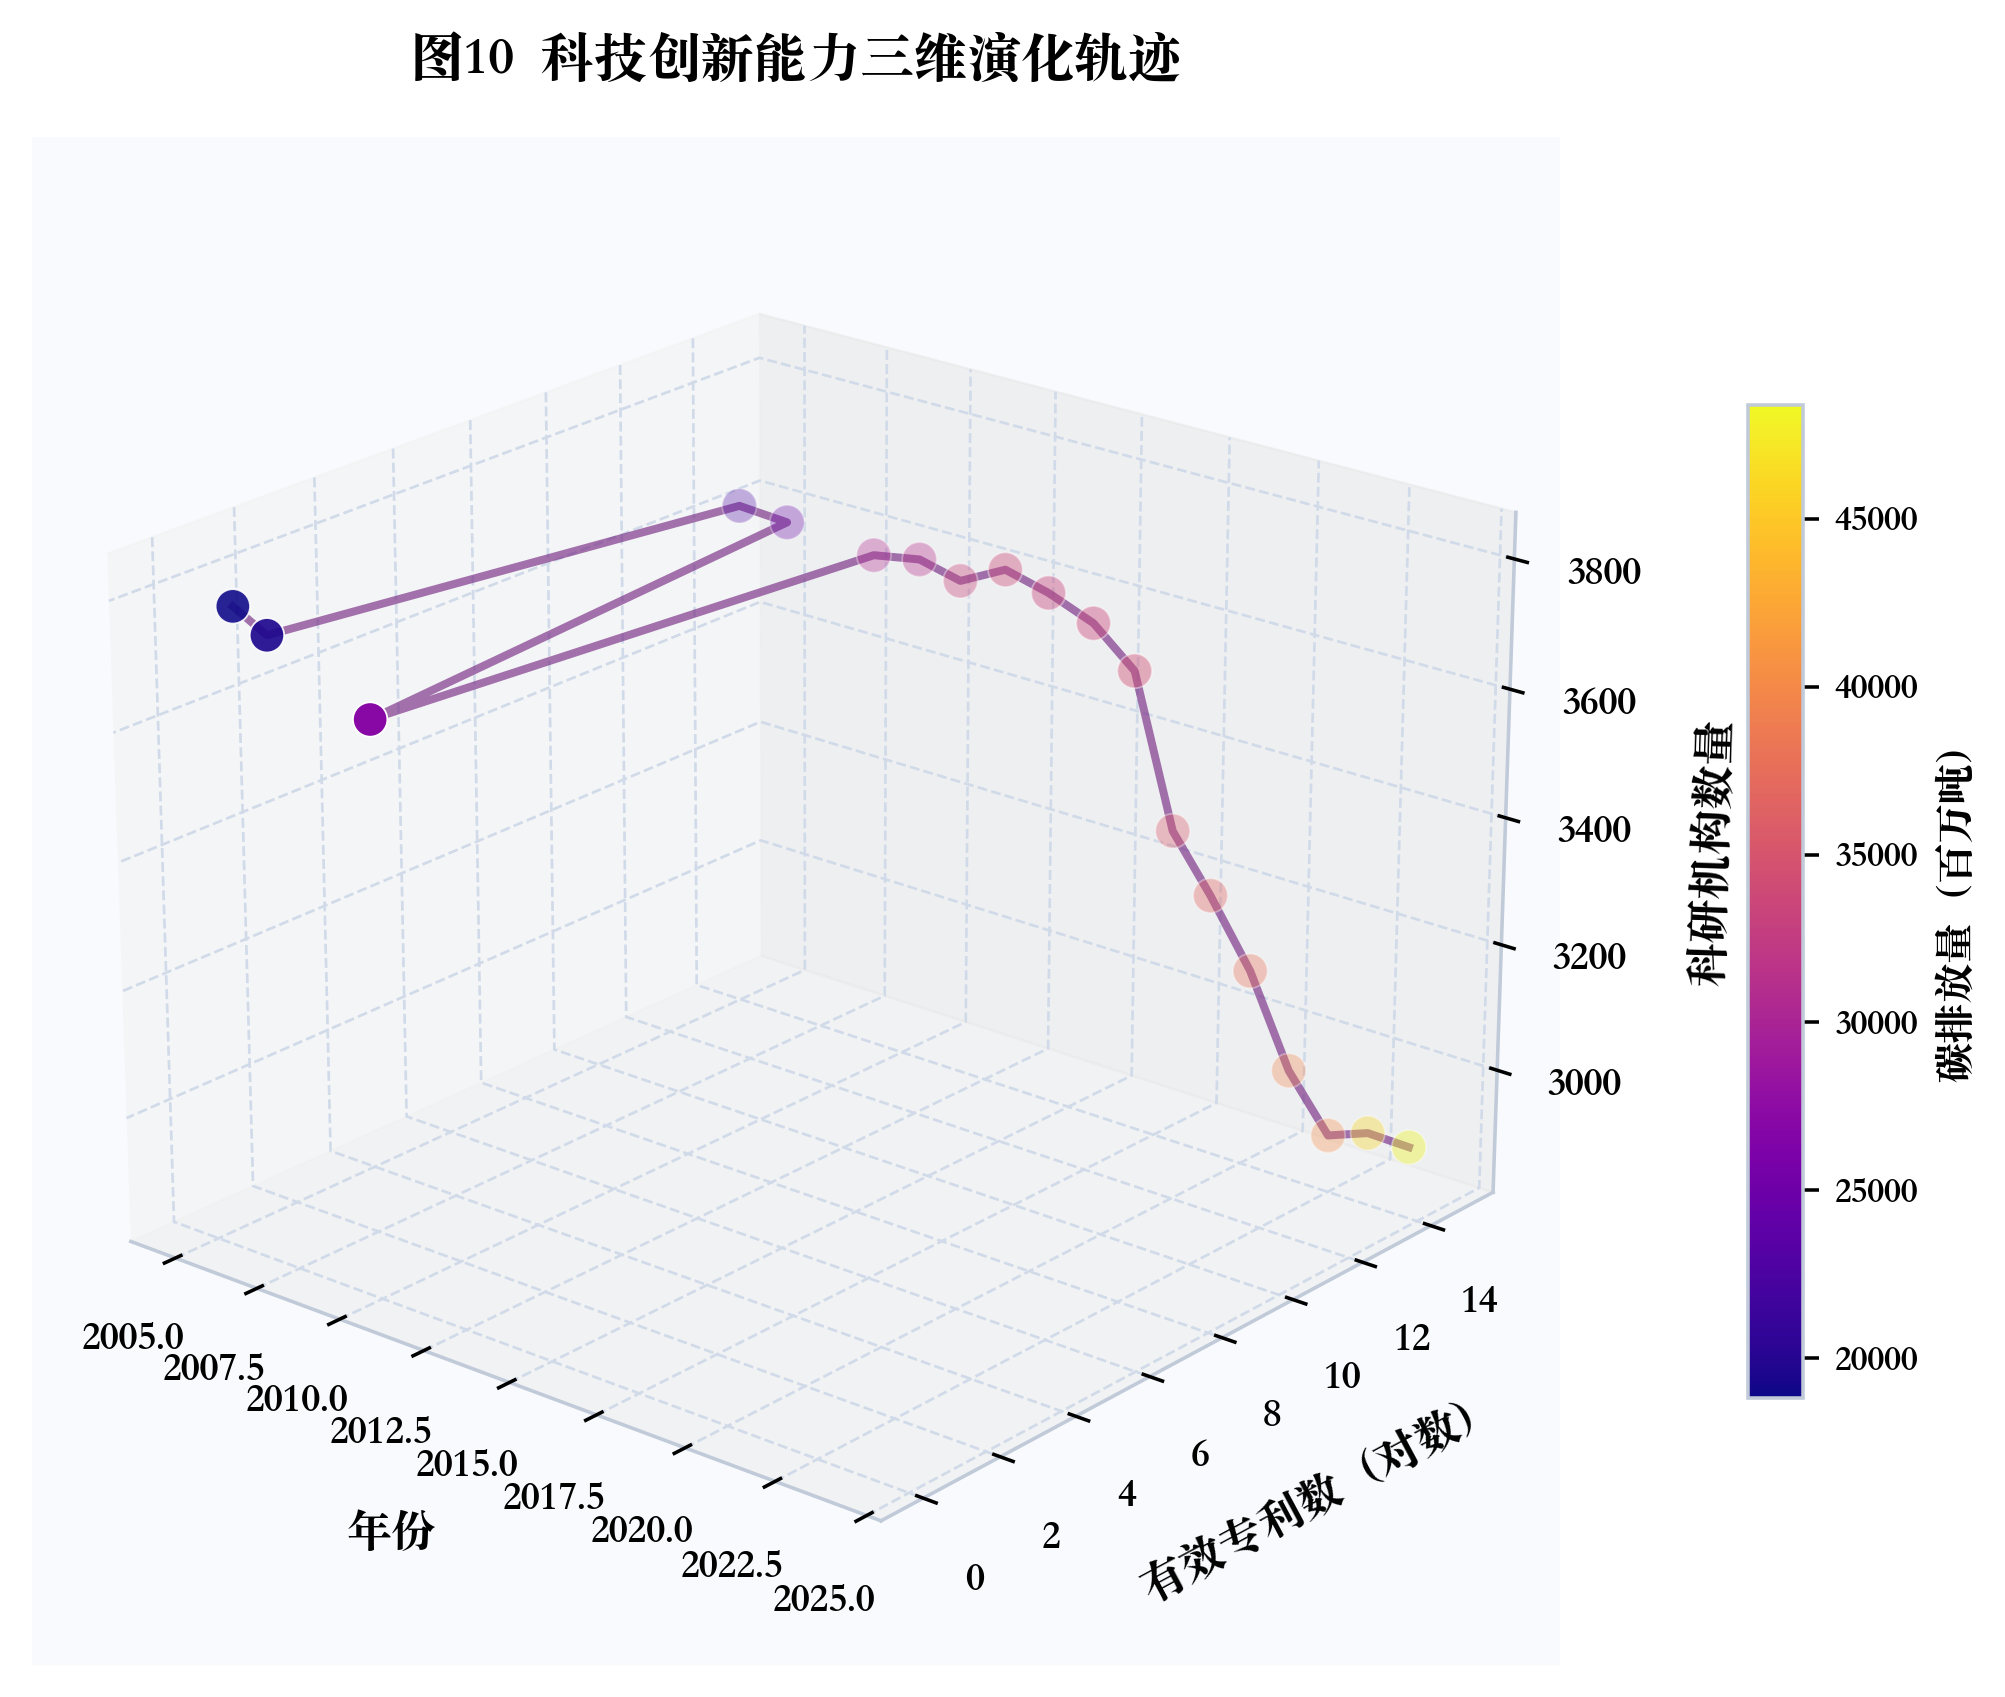
\includegraphics[width=0.78\textwidth]{../outputs/figures/Fig10_innovation_capacity.png}
    \captionof{figure}{技术创新能力三维轨迹图}
    \label{fig:innovation_3d}
\end{center}
从图\ref{fig:innovation_3d}可见，专利、科研机构与碳排放的三维轨迹更接近“缓释效应”特征，即技术因素通过时间积累逐步改变边际排放，而非在短期内直接逆转总量趋势。

\begin{table}[H]
\centering
\caption{扩展STIRPAT主要弹性系数估计结果}
\label{tab:stirpat_coeff}
\begin{tabular}{cccc}
\midrule
Affluence & 0.5882 & -0.9264 & 2.1027 \\
Energy Intensity & 0.0401 & -1.7464 & 1.8266 \\
Coal Share & 3.3791 & 0.0469 & 6.7112 \\
Urbanization & 2.7347 & -5.0452 & 10.5146 \\
Technology & -0.0018 & -0.0086 & 0.0049 \\
Industrial Structure & 0.7915 & -2.2662 & 3.8492 \\
\bottomrule
\end{tabular}
\end{table}

\subsection{预测与情景模拟}
本节聚焦两个问题：在小样本国家级时序中何种模型更稳健，以及不同政策强度下峰值水平可被压低到何种区间。

\begin{center}
    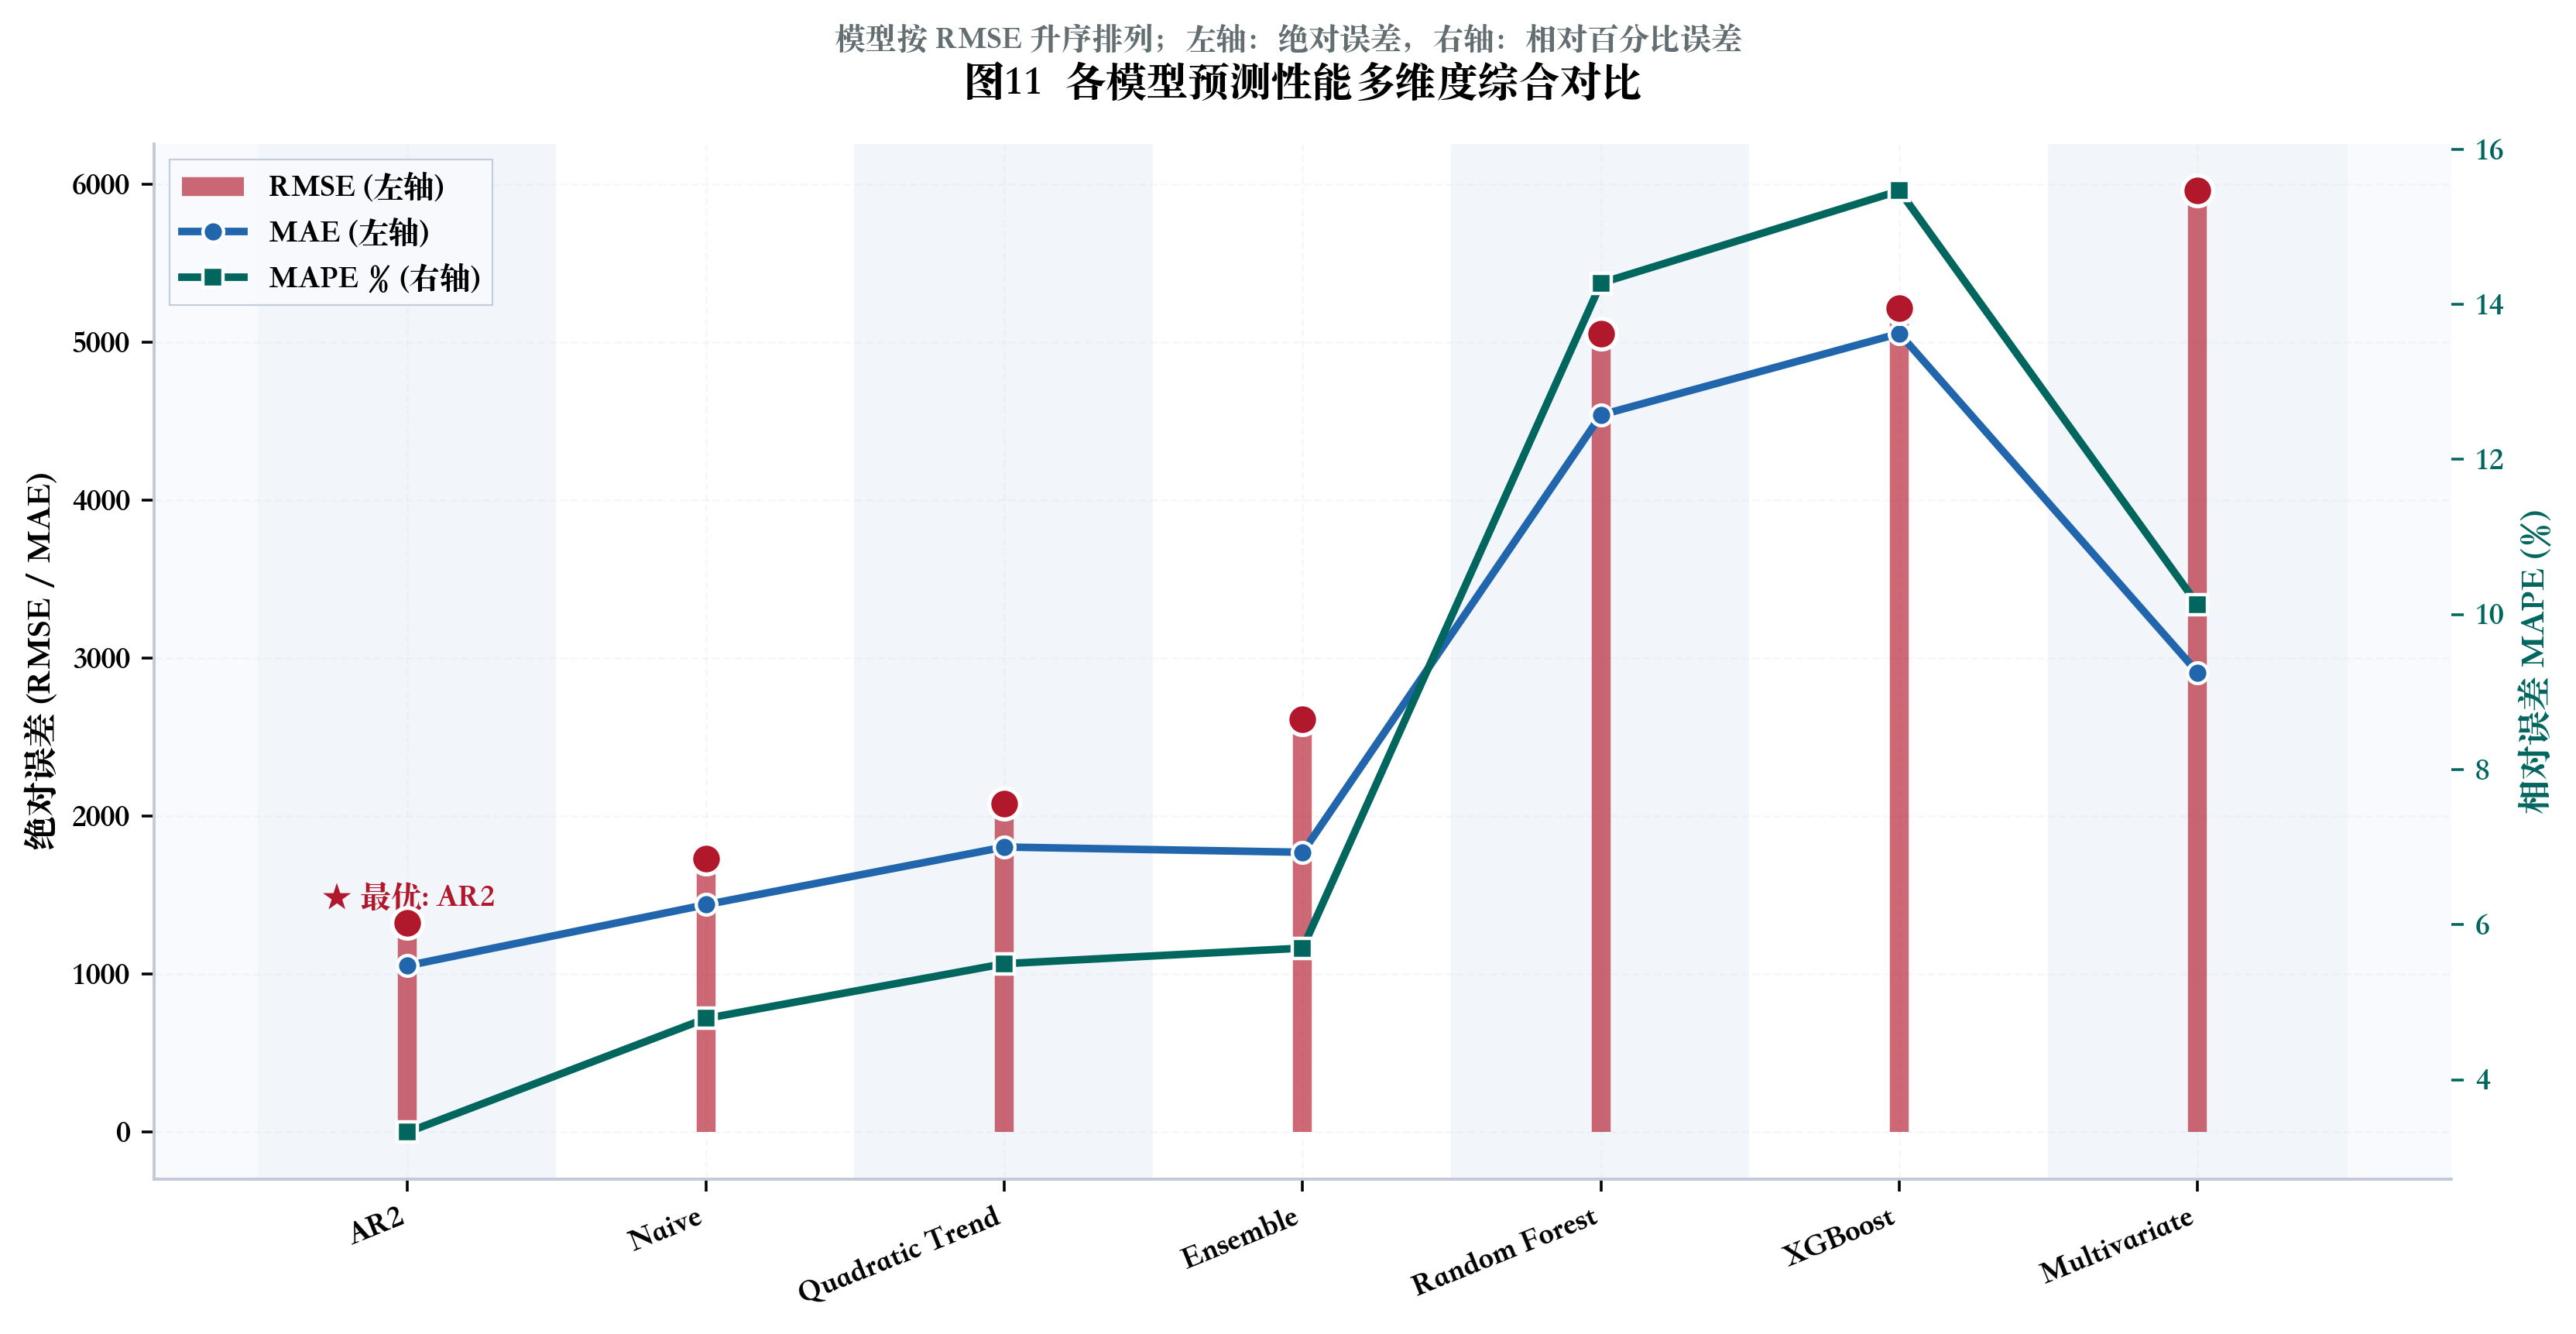
\includegraphics[width=0.80\textwidth]{../outputs/figures/Fig11_model_performance.png}
    \captionof{figure}{多模型滚动预测误差比较}
    \label{fig:model_perf}
\end{center}
图\ref{fig:model_perf}显示，在统一可比窗口下，AR2 模型误差最低（RMSE=1323.36，MAPE=3.32\%），朴素模型次之；二次趋势模型表现尚可。然而，值得关注的现象是，引入高维特征或多树集成的复杂模型出现了显著的性能崩塌：XGBoost（RMSE=5214.83）与随机森林（RMSE=5054.08）的误差远高于传统基准，多变量回归也表现不佳。这一“复杂度失效”现象并非算法本身的缺陷，而是由国家级时序样本量极小（仅18期观测值）导致的严重过拟合——树模型无法在极少样本中提取稳健的分裂规则，导致外推方差急剧放大。该结果以直观的对比形式，有力地支撑了本文“模型适配性优先于模型复杂度”的核心论断。

单位根检验表明序列为 I(1) 过程，解释了为何依赖序列动态的 AR 模型更稳健，而水平拟合的高复杂度模型易累积误差。
\begin{center}
    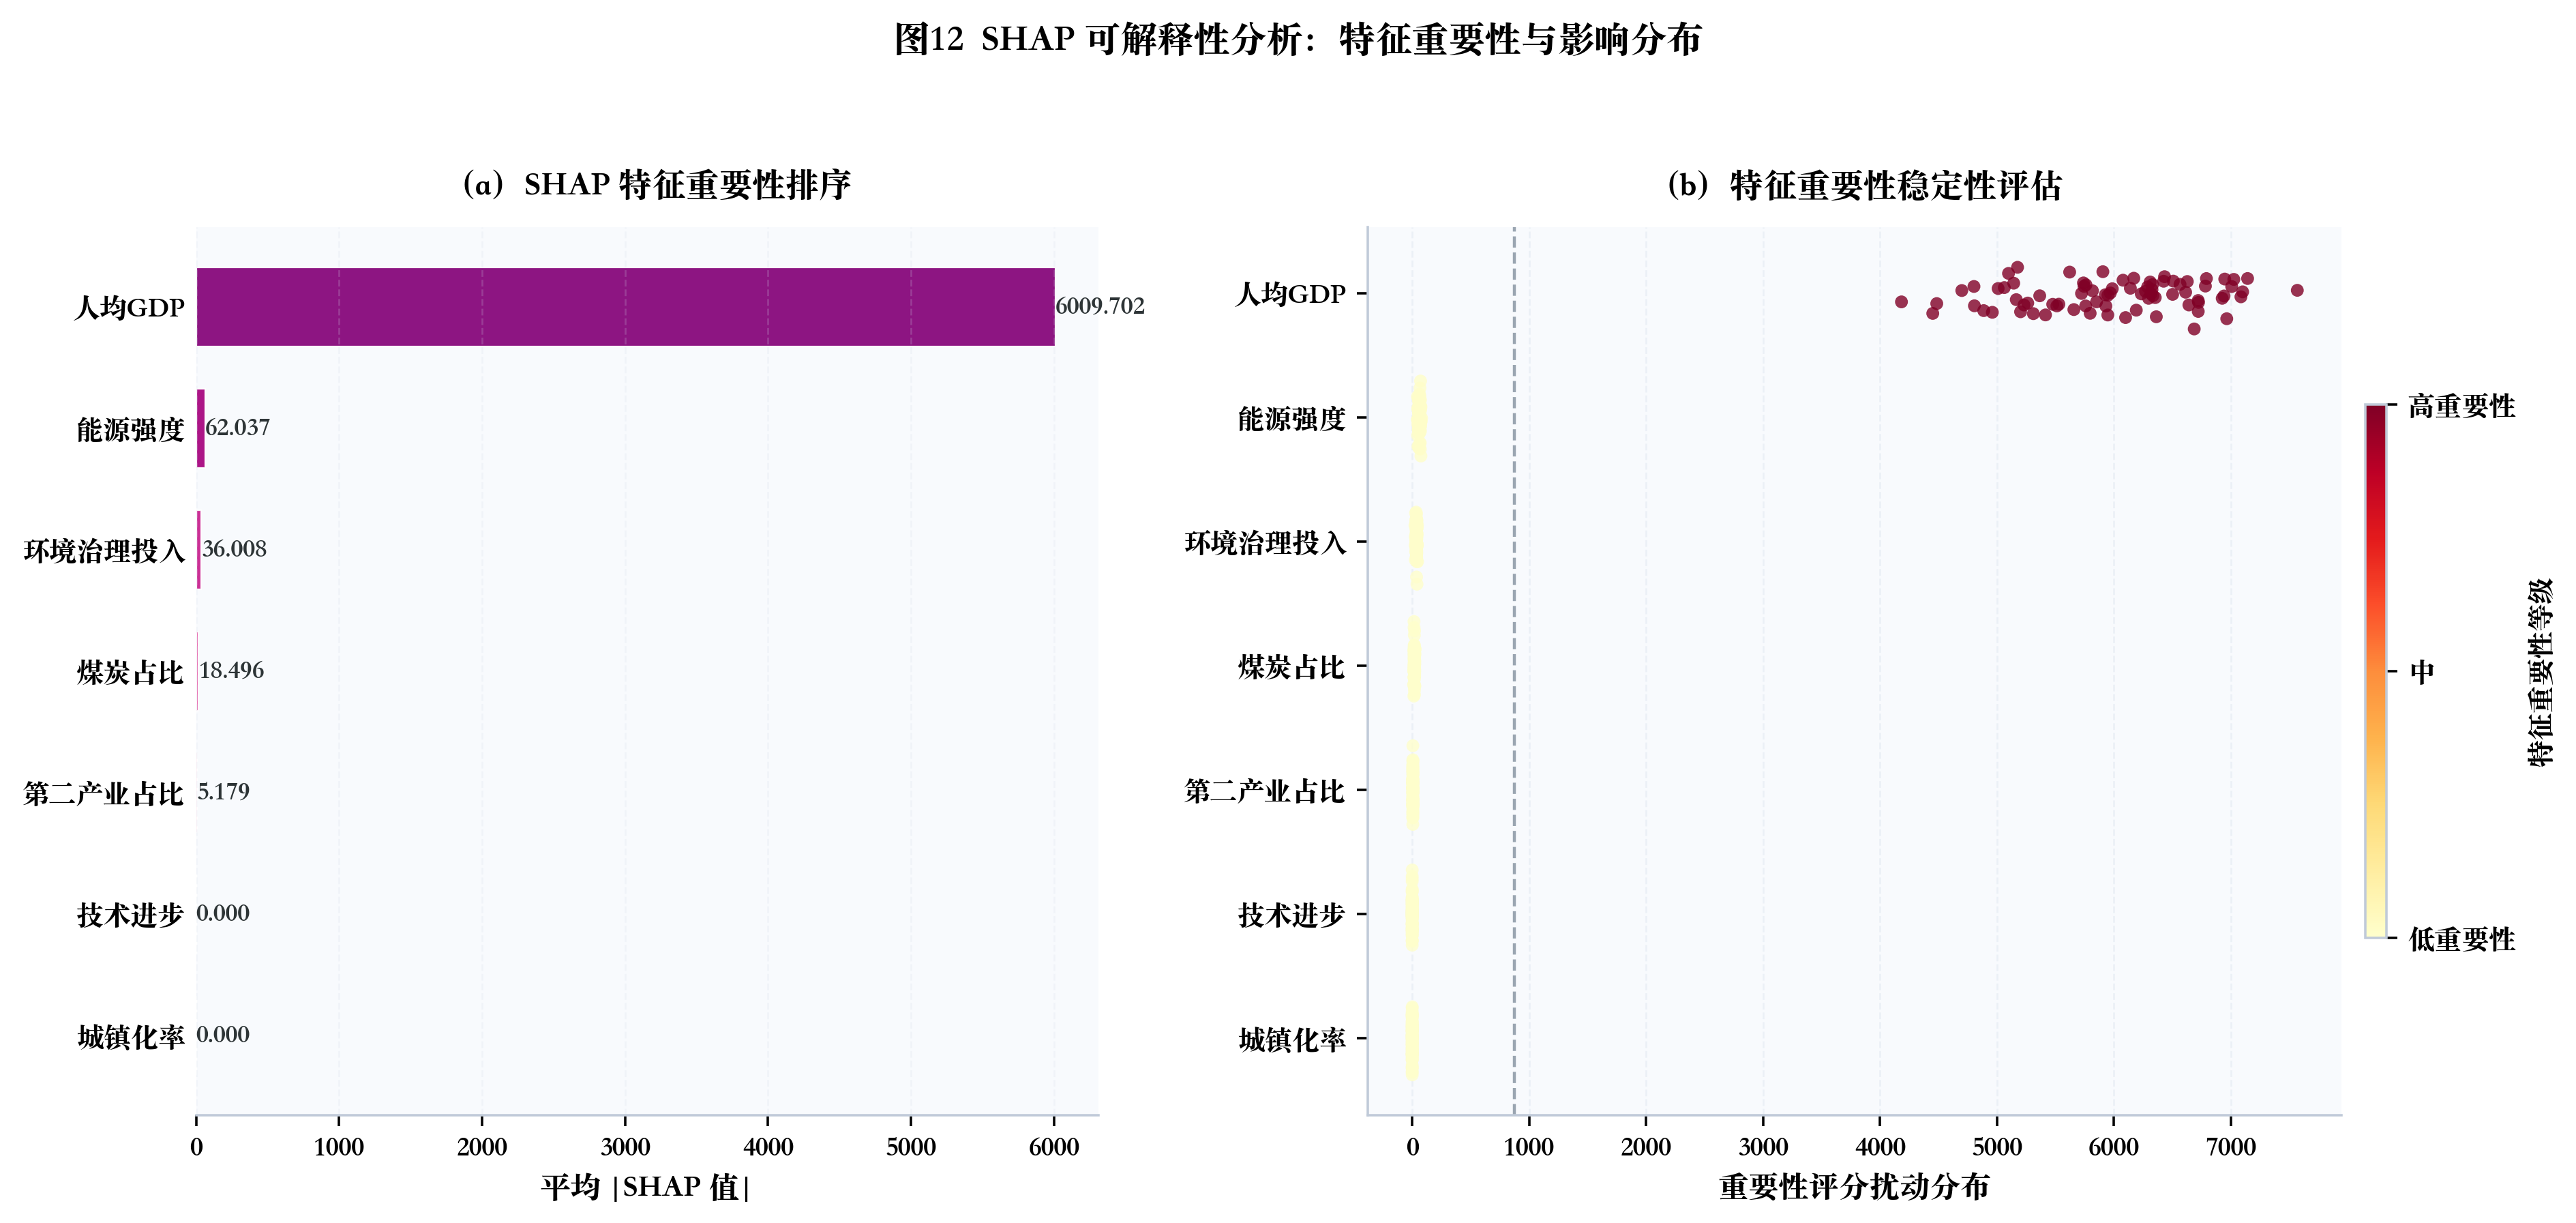
\includegraphics[width=0.92\textwidth]{../outputs/figures/Fig12_shap_summary.png}
    \captionof{figure}{基于XGBoost模型的特征重要性SHAP分析}
    \label{fig:shap}
\end{center}
图\ref{fig:shap}a）展示了基于 XGBoost 模型的真实 SHAP 全局特征重要性排序。结果显示，人均 GDP 的平均绝对 SHAP 值远超其他变量，呈现出明显的``主导地位''，而城镇化率与技术进步的特征重要性为 0。

这一结果看似与前文STIRPAT中“煤炭占比最显著”的结论相左，实则反映了小样本下复杂模型在特征选择上的局限性。具体而言，在仅有18期的宏观时序中，人均GDP与碳排放高度共线。XGBoost在节点分裂时，直接被该主导特征主导，导致其他变量的特征重要性被完全掩盖。

反观前文的 STIRPAT 模型，其本质是多元线性回归，强制要求所有变量在同一方程中竞争解释力（控制了共线性与规模效应）。正是这种机制，识别出了煤炭占比的独立正向弹性。此外，SHAP结果中城镇化与技术进步重要性为0，也与STIRPAT中二者未达统计显著的结果相互印证。

综合来看，SHAP分析从侧面证实了前文的判断：小样本下盲目追求算法复杂度，不仅损害预测外推性，还容易导致机制识别的失真。

\begin{table}[H]
\centering
\caption{主要模型预测误差比较}
\label{tab:model_perf}
\begin{tabular}{cccc}
\toprule
模型 & RMSE & MAE & MAPE(\%) \\
\midrule
AR2 & 1323.36 & 1054.50 & 3.32 \\
Naive & 1732.09 & 1440.44 & 4.79 \\
Quadratic Trend & 2081.10 & 1805.35 & 5.50 \\
Ensemble & 2612.10 & 1772.16 & 5.70 \\
Random Forest & 5054.08 & 4540.33 & 14.27 \\
XGBoost & 5214.83 & 5056.28 & 15.47 \\
Multivariate & 5959.72 & 2909.50 & 10.13 \\
\bottomrule
\end{tabular}
\end{table}

\begin{center}
    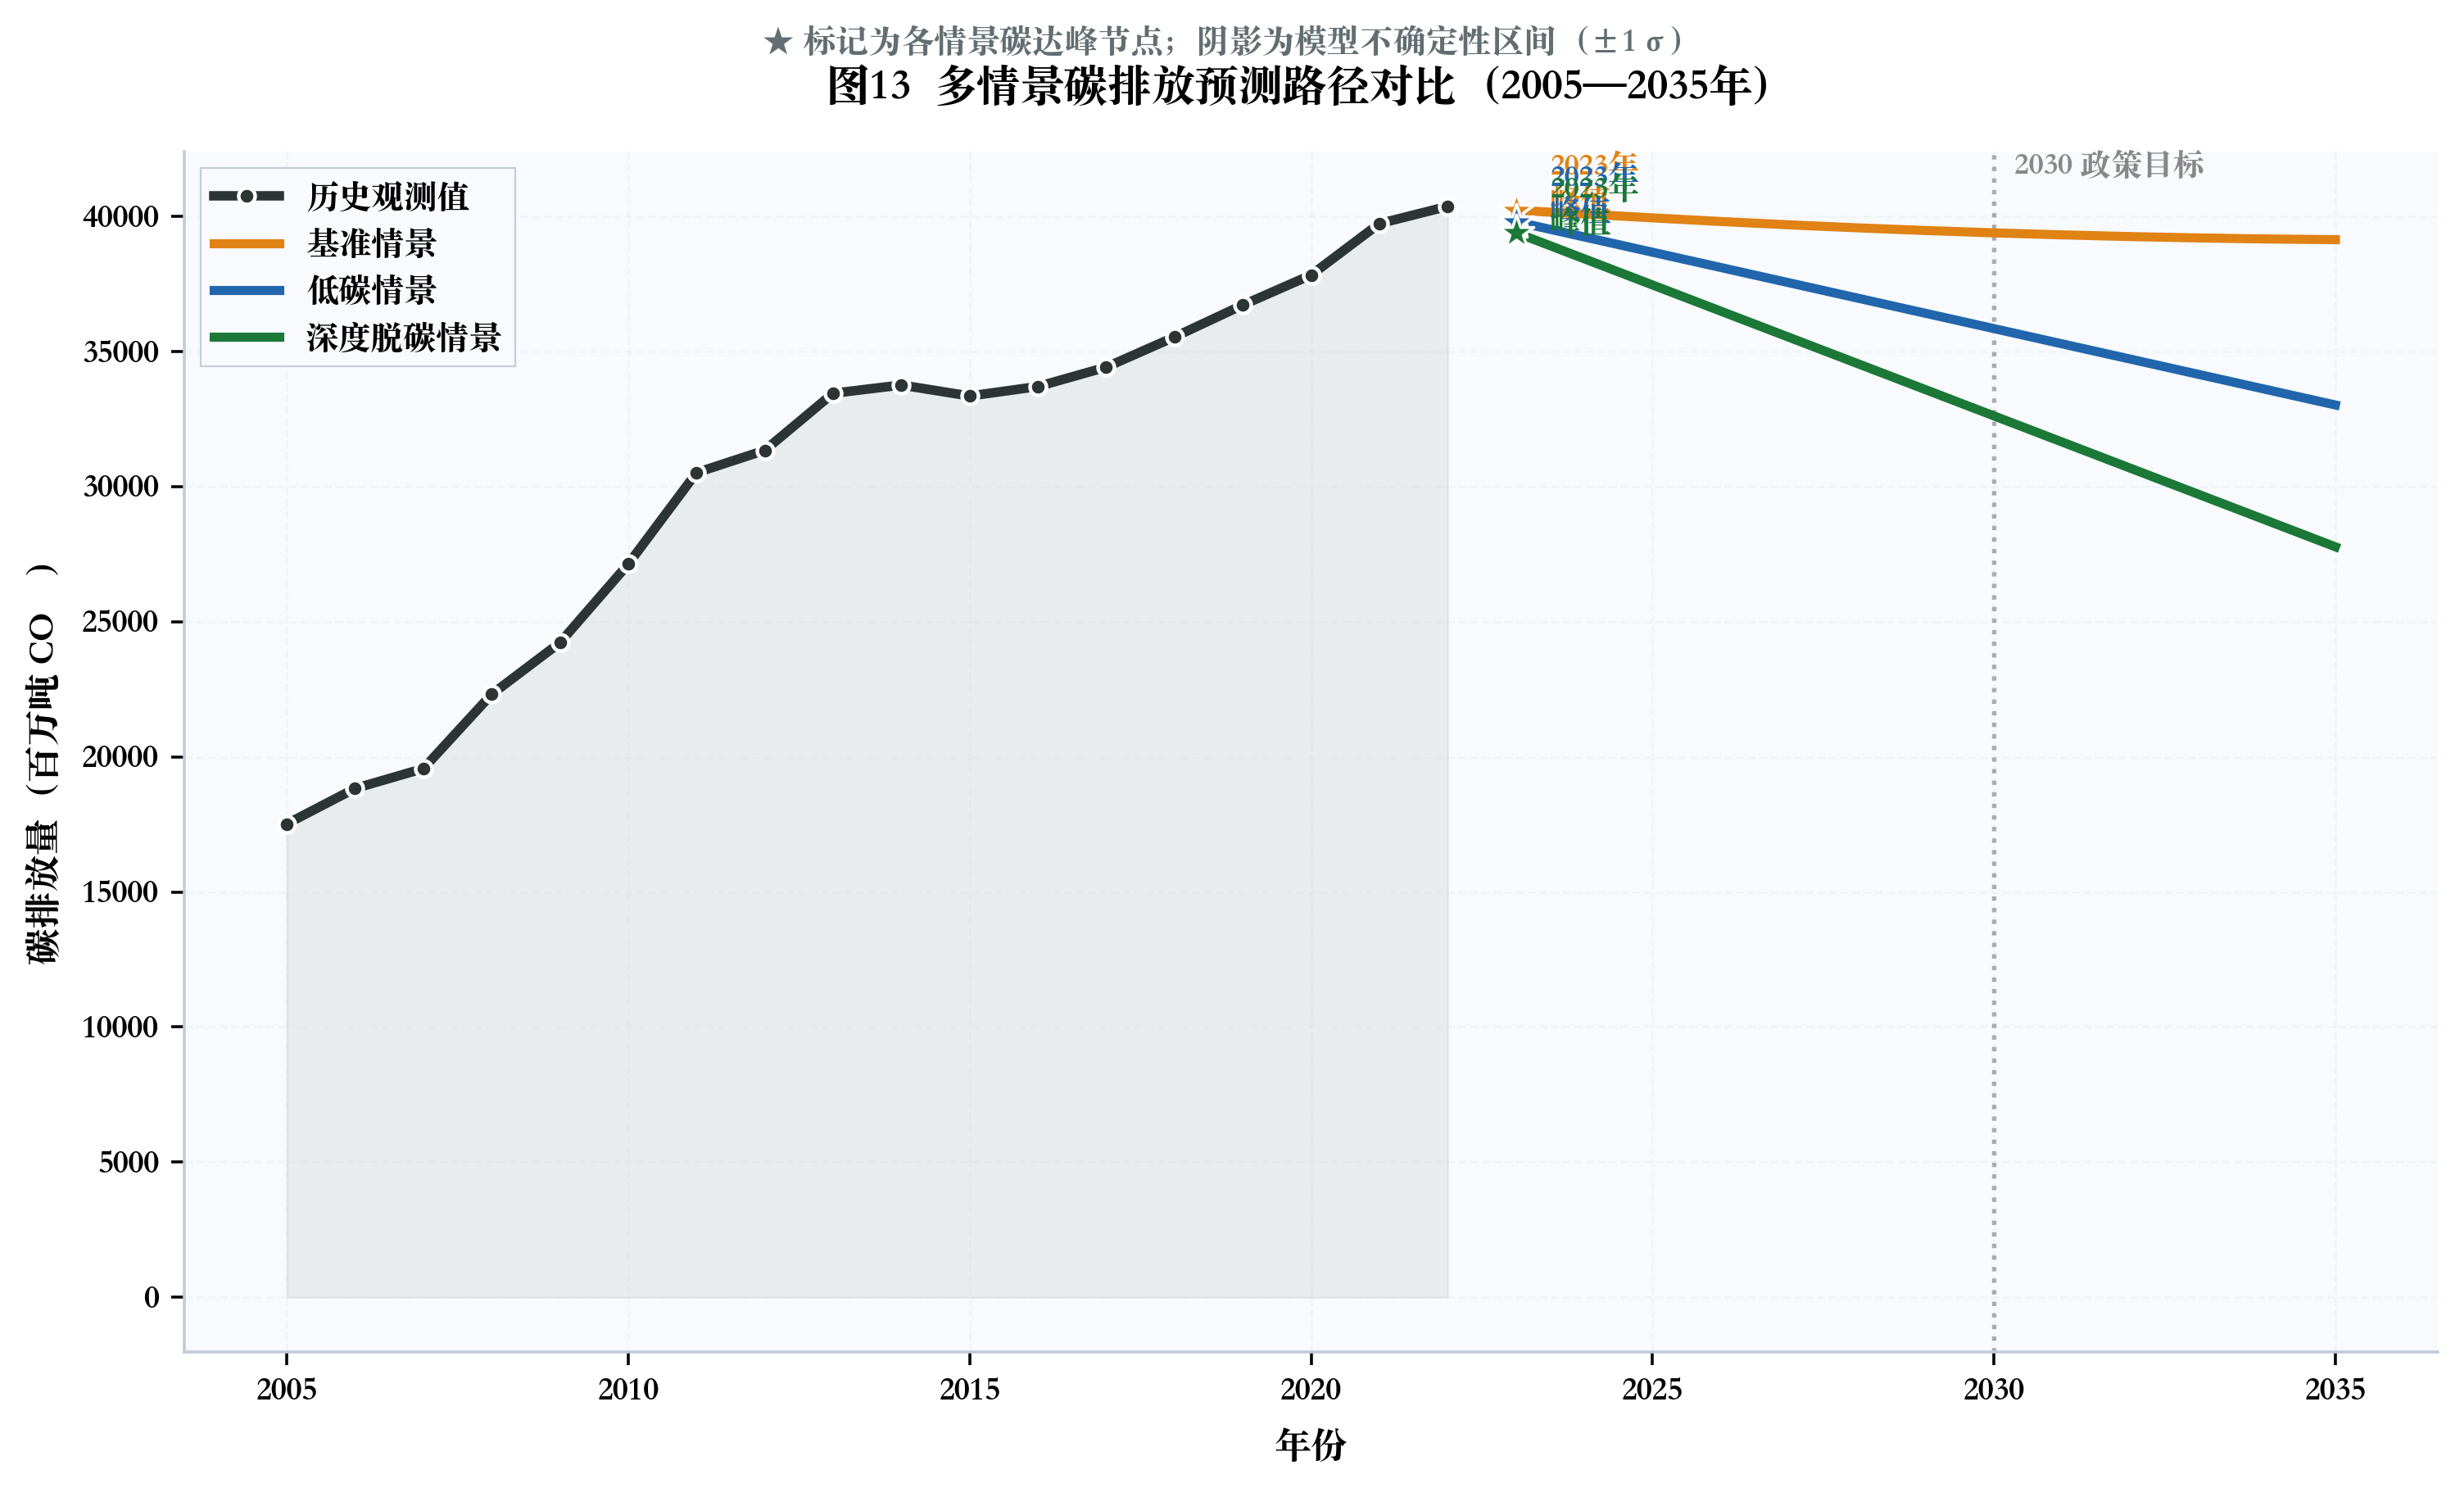
\includegraphics[width=0.82\textwidth]{../outputs/figures/Fig13_scenario_paths.png}
    \captionof{figure}{不同情景下碳排放路径预测比较（2025—2035）}
    \label{fig:scenario_paths}
\end{center}
从图\ref{fig:scenario_paths}可以看到，基准、低碳和深度脱碳三类情景在2025—2035年形成明显分叉。到2035年，基准约39127.33 Mt，低碳约33013.06 Mt，深度脱碳约27766.48 Mt。

\begin{center}
    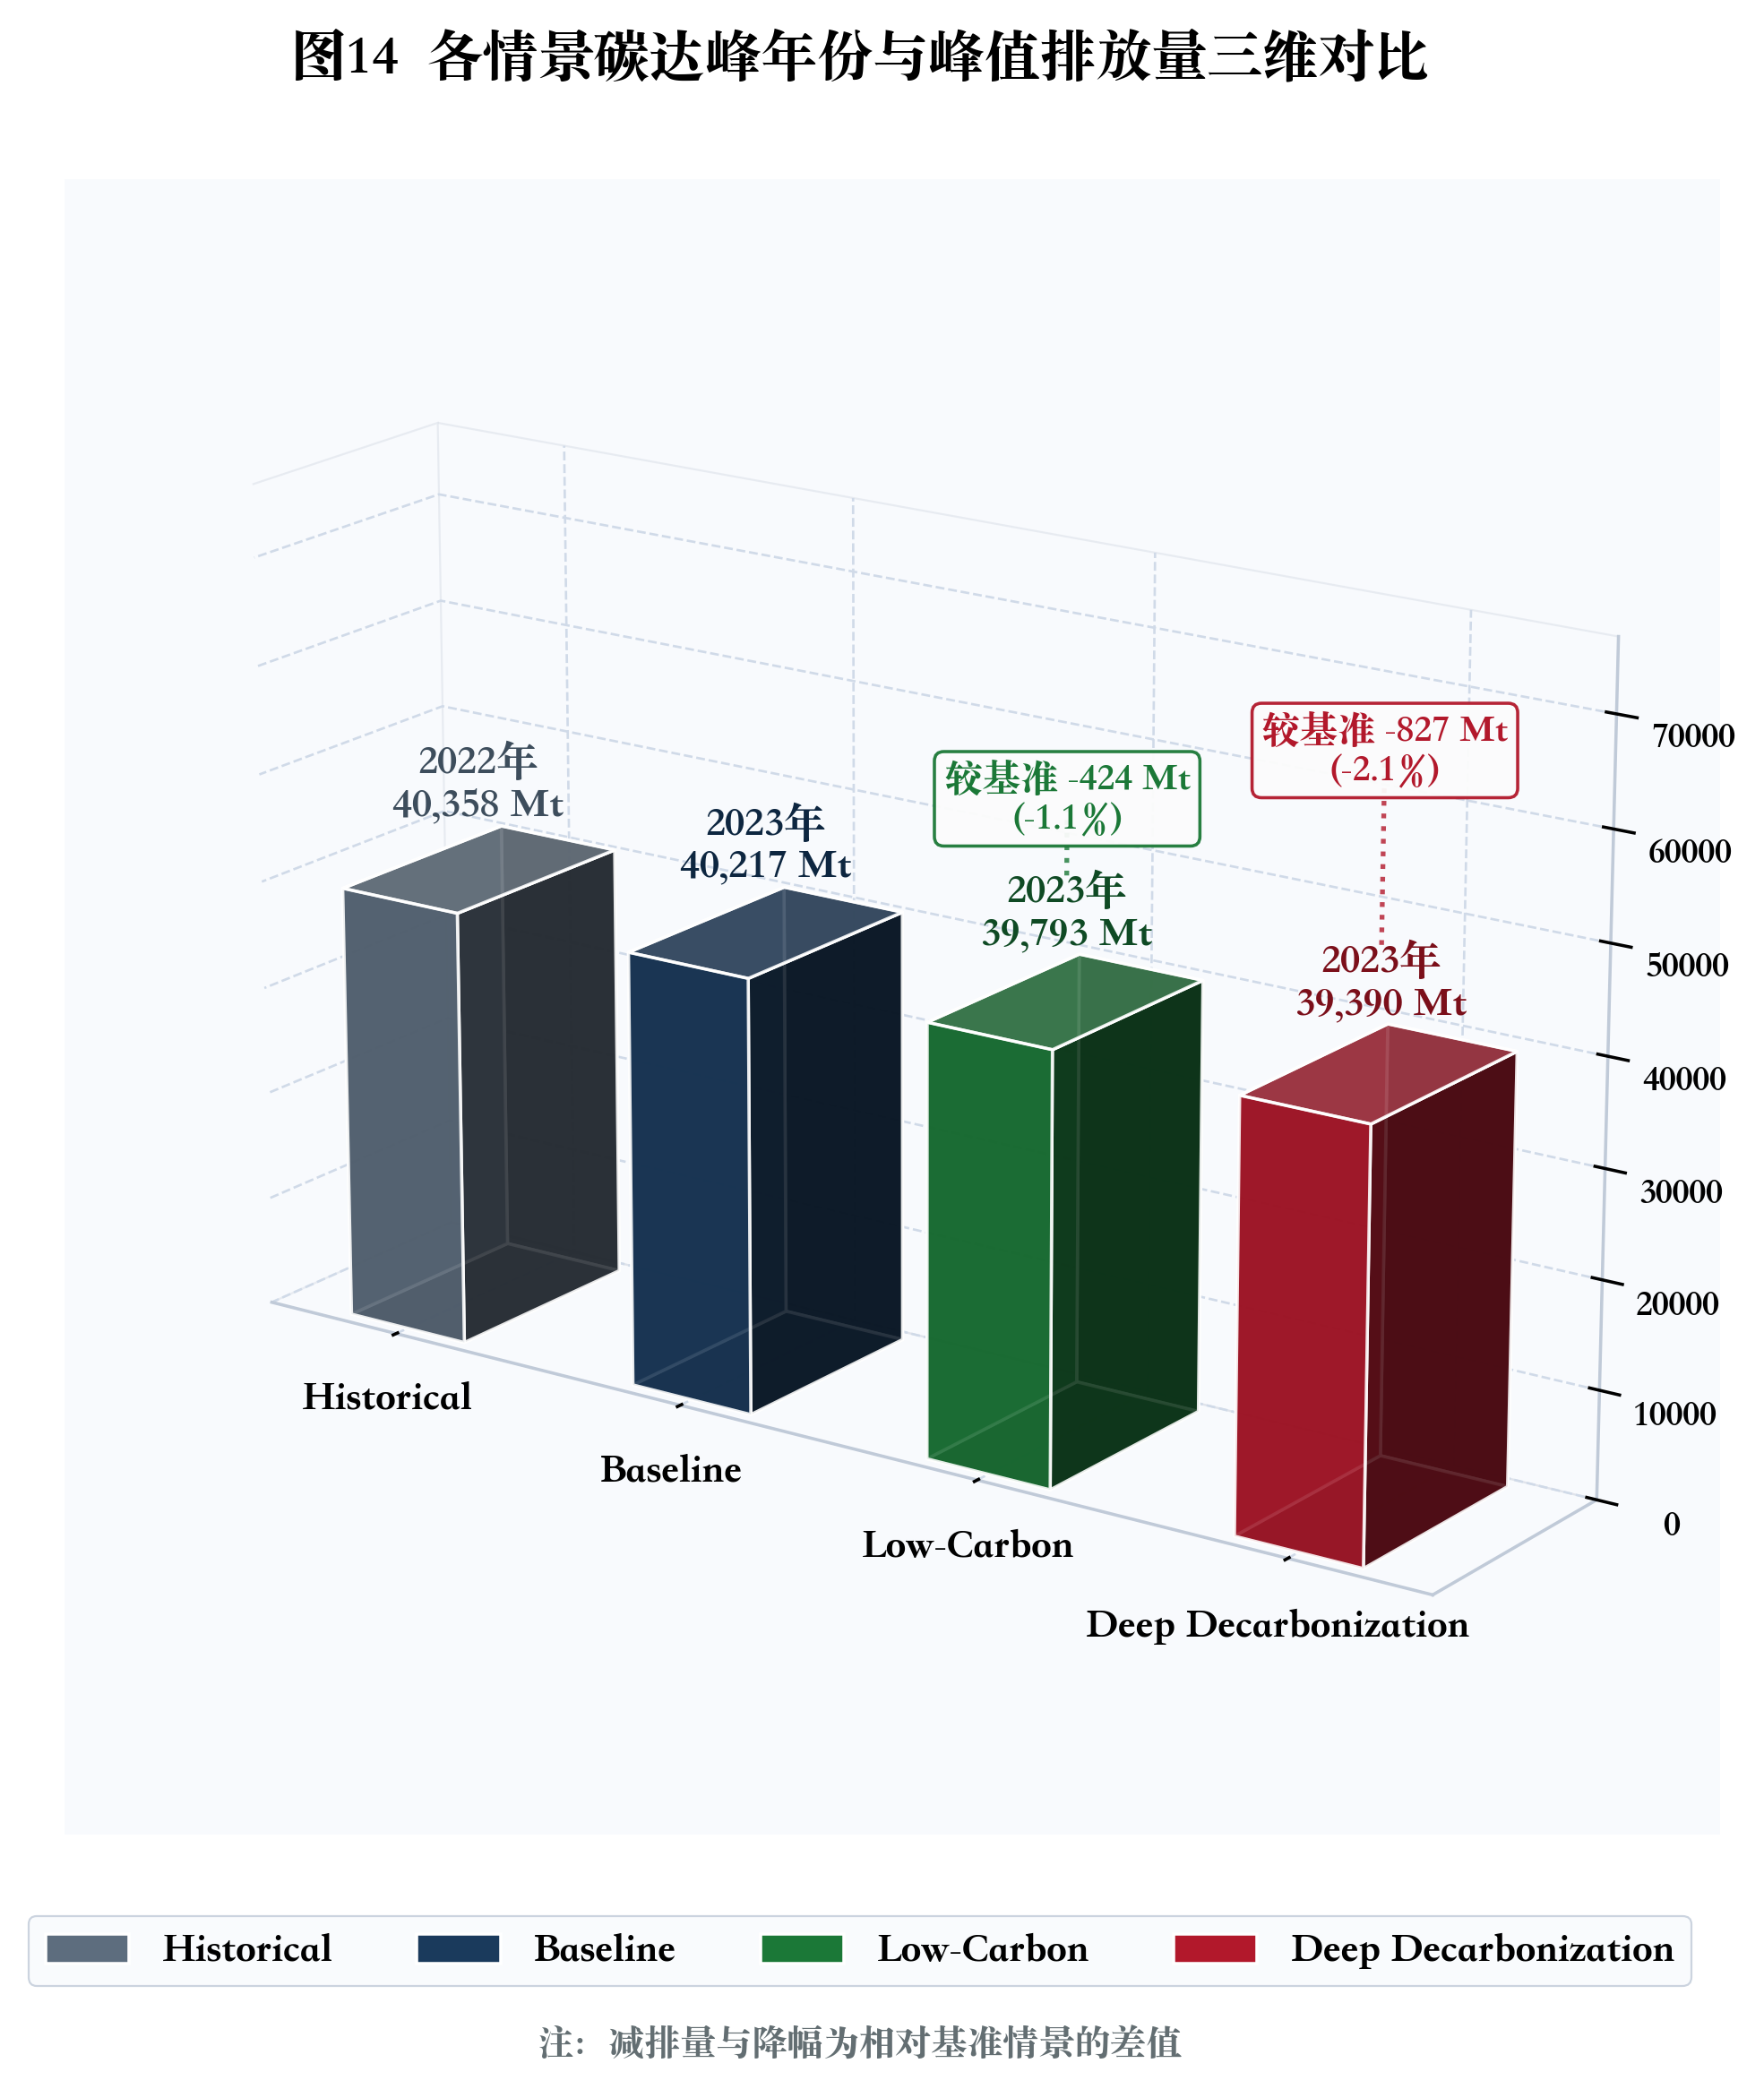
\includegraphics[width=0.80\textwidth]{../outputs/figures/Fig14_peak_bubble.png}
    \captionof{figure}{不同情景峰值年份与峰值规模三维比较}
    \label{fig:peak_3d}
\end{center}
图\ref{fig:peak_3d}显示，历史观测路径峰值约40358.26 Mt（2022年），三类政策情景下峰值均低于该历史高点。

\begin{table}[H]
\centering
\caption{多情景核心参数设定表}
\label{tab:scenario_params}
\small 
\begin{tabularx}{\textwidth}{lXXX} 
\toprule
情景 & GDP年均增速(\%) & 煤炭占比年均变动(百分点) & 能源强度年均下降(\%) \\
\midrule
Baseline & 5.0 & -0.6 & 2.3 \\
Low-Carbon & 4.6 & -1.1 & 2.8 \\
Deep Decarbonization & 4.4 & -1.6 & 3.6 \\
\bottomrule
\end{tabularx}

{\footnotesize 注：参数区间参考《“十四五”现代能源体系规划》与国家统计局近年宏观运行区间设定。}
\end{table}

\begin{table}[H]
\centering
\caption{2035年不同情景碳排放预测结果}
\label{tab:scenario_2035}
\begin{tabular}{cc}
\toprule
情景 & 2035年碳排放(Mt) \\
\midrule
Baseline & 39127.33 \\
Low-Carbon & 33013.06 \\
Deep Decarbonization & 27766.48 \\
\bottomrule
\end{tabular}
\end{table}

表\ref{tab:scenario_params}给出了三类情景的参数设定。参数锚定于国家能源结构优化与能效提升目标导向，并结合近年宏观运行区间设定，用于构造可比的政策强度梯度。表\ref{tab:scenario_2035}与图\ref{fig:scenario_paths}、图\ref{fig:peak_3d}相互印证：在能源替代、产业升级、技术扩散三方面同步加力，可将未来峰值压至更低平台，进而降低长期减排成本。
